%!TEX root = thesis.tex

\chapter{Further Results}\label{furtherResults}

\section{Building Energy Analysis}
\label{s:buildingResults}
	
	As the building energy results are available for every hour of the year, they can be visualised in greater detail than the overall results that include the PV electricity production given in Section \ref{s:baseCase}. 

	The optimal configurations of the ASF can be visualised using carpet-plots. For a classical building analysis this was done for every hour of the year. Figures \ref{f:DIVAx} and \ref{f:DIVAy} show the optimizing altitude and azimuth angles for heating, cooling, lighting and total building energy demand. In figure \ref{f:DIVAx}, darker colours represent closed positions, whereas brighter colours correspond to open positions. To optimize heating and lighting, open positions (corresponding to large altitude angles) are favourable, cooling is optimized by using closed positions (corresponding to small altitude angles). The overall optimized solutions follow the corresponding patterns at the hours of importance. The azimuth angles in figure \ref{f:DIVAy} correspond to the deviation from the facade normal. For a south facing facade, this means an angle with a positive sign represents the panels facing towards south-east (bright colours), whereas negative angles represent the panels facing towards south-west (dark colours). It can be seen that for heating and lighting, the facade takes positions that let the sun in, whereas for cooling the facade follows a sun-tracking pattern which prevents radiation to enter the room. 

	\begin{figure*}
		\begin{center}
		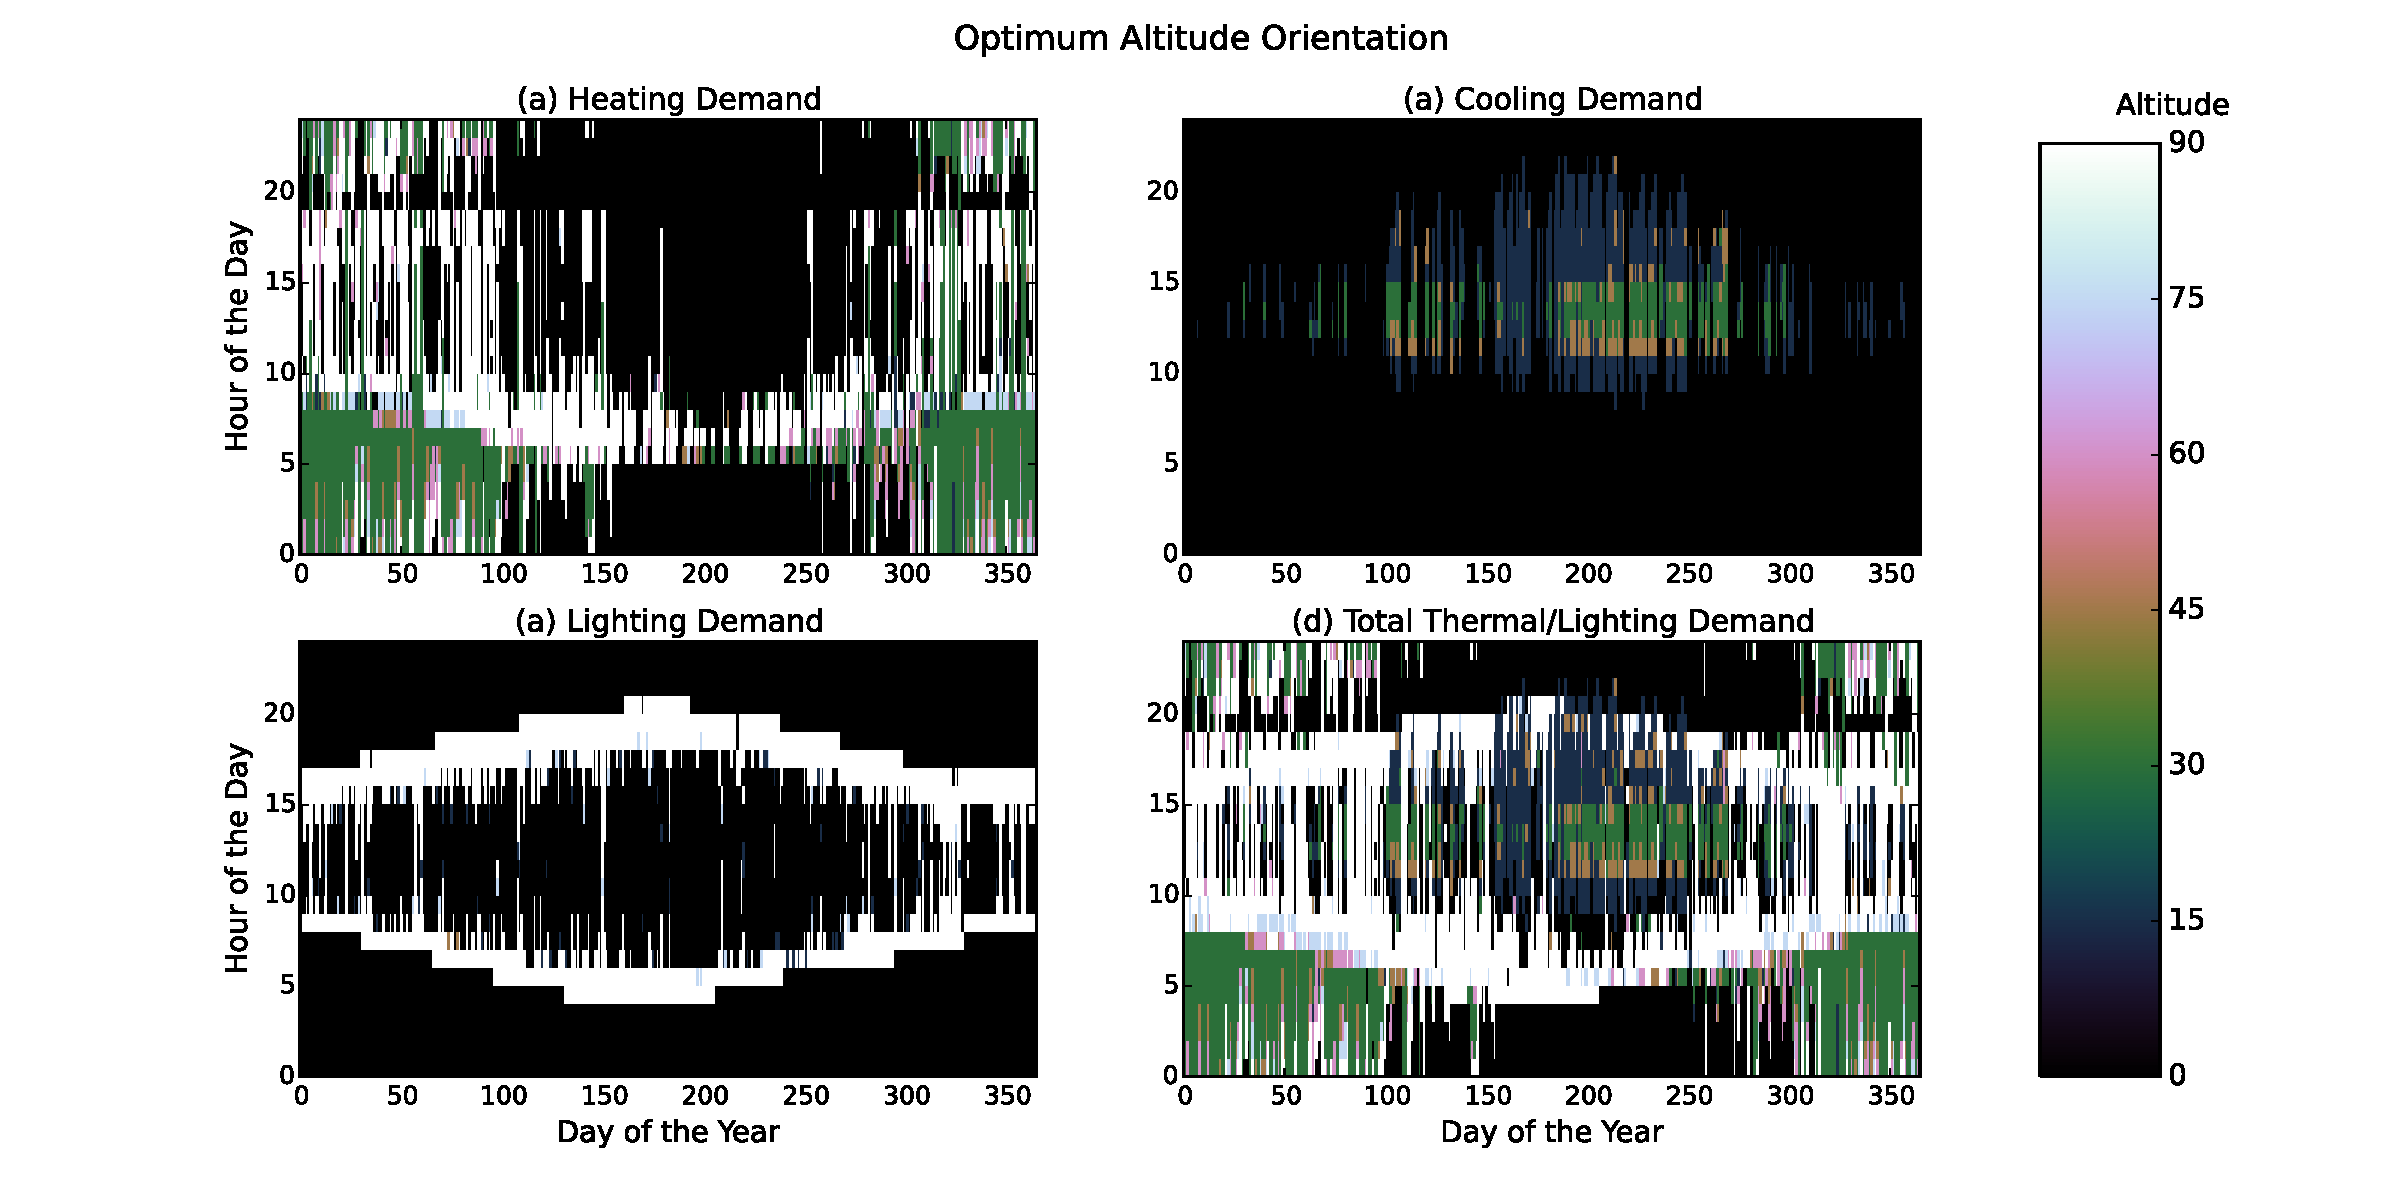
\includegraphics[width=\textwidth, trim= 0cm 0cm 0cm 0cm,clip]{DIVAx2}
		\caption{Carpet plots detailing the optimal altitude angles to minimise the (a) heating demand, (b) cooling demand, (c) lighting demand, and (d) total building energy demand. Darker colours represent closed positions, whereas brighter colors correspond to open positions. To optimize heating and lighting, open positions are favorable, cooling is optimized by using closed positions.}
		\label{f:DIVAx}
		\end{center}
	\end{figure*}


	\begin{figure*}
		\begin{center}
		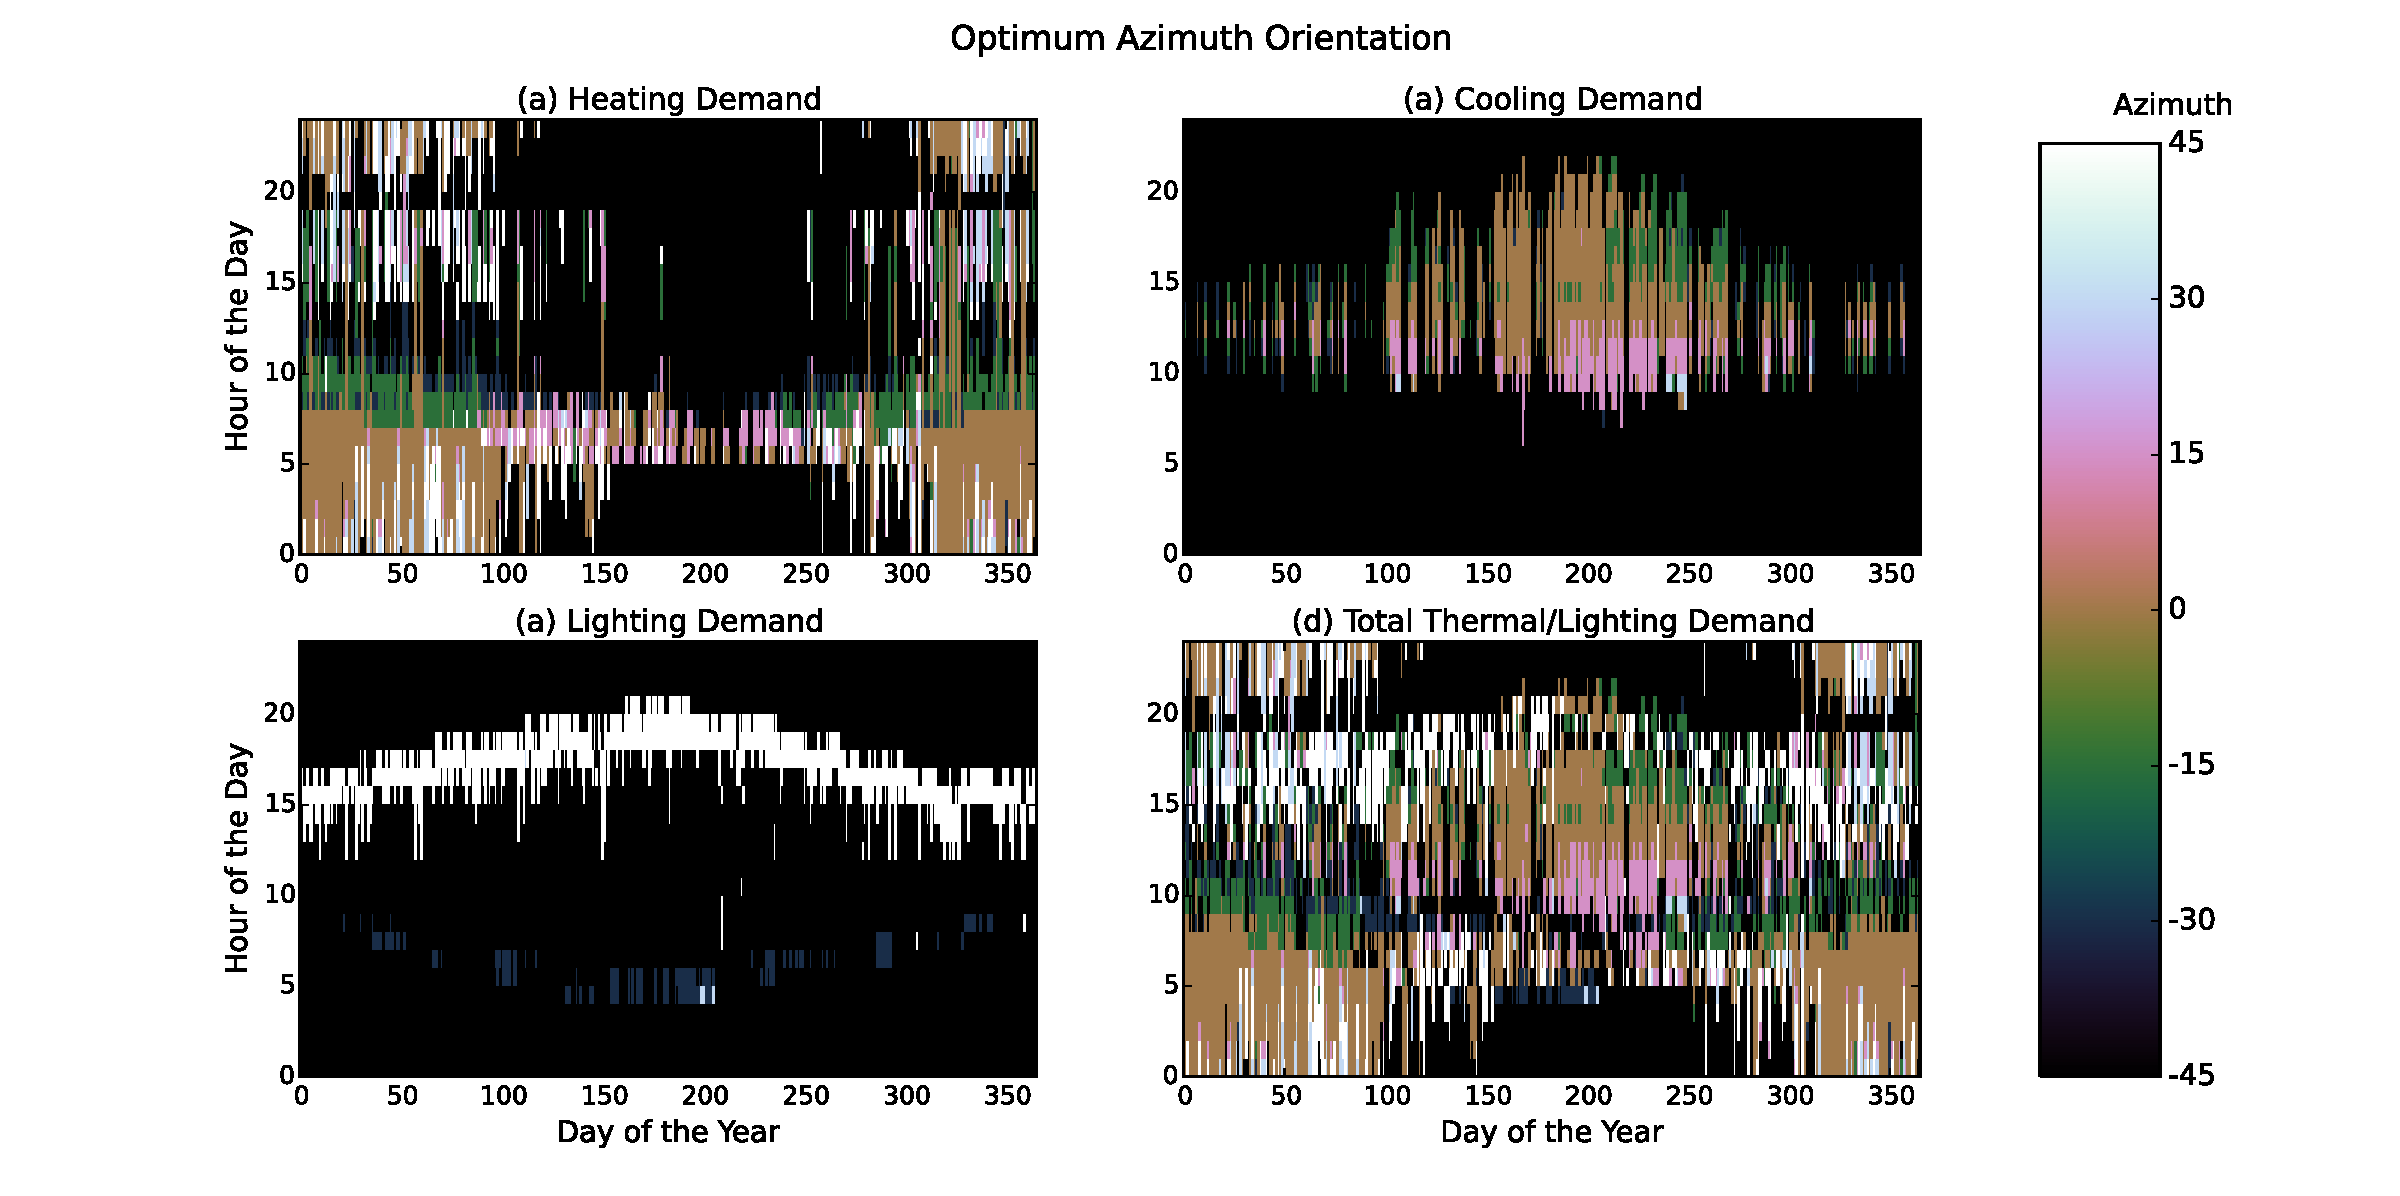
\includegraphics[width=\textwidth, trim= 0cm 0cm 0cm 0cm,clip]{DIVAy2}
		\caption{Carpet plots detailing the optimal azimuth angles to minimise the (a) heating demand, (b) cooling demand, (c) lighting demand, and (d) total building energy demand. Cooling is minimized by blocking the sun, whereas lighting and heating are minimized by opening the facade to let the insolation in.}
		\label{f:DIVAy}
		\end{center}
	\end{figure*}

	Figure \ref{f:DIVAe} depicts the corresponding energy demand of the building for the whole year corresponding to the optimum positions presented in figures \ref{f:DIVAx} and \ref{f:DIVAy}. It can be seen that heating is most needed during the winter and in the morning, whereas cooling is mainly apparent in summer afternoons. Lighting on the other hand is most important in the evenings and at times where there is not much sun. In the combined plot, this behavior can be seen clearly as well, the main overlaps of different building energy consumptions take place during winter between heating and lighting in the morning and in the evening, and between cooling and lighting during summer evenings. 

	\begin{figure*}
		\begin{center}
		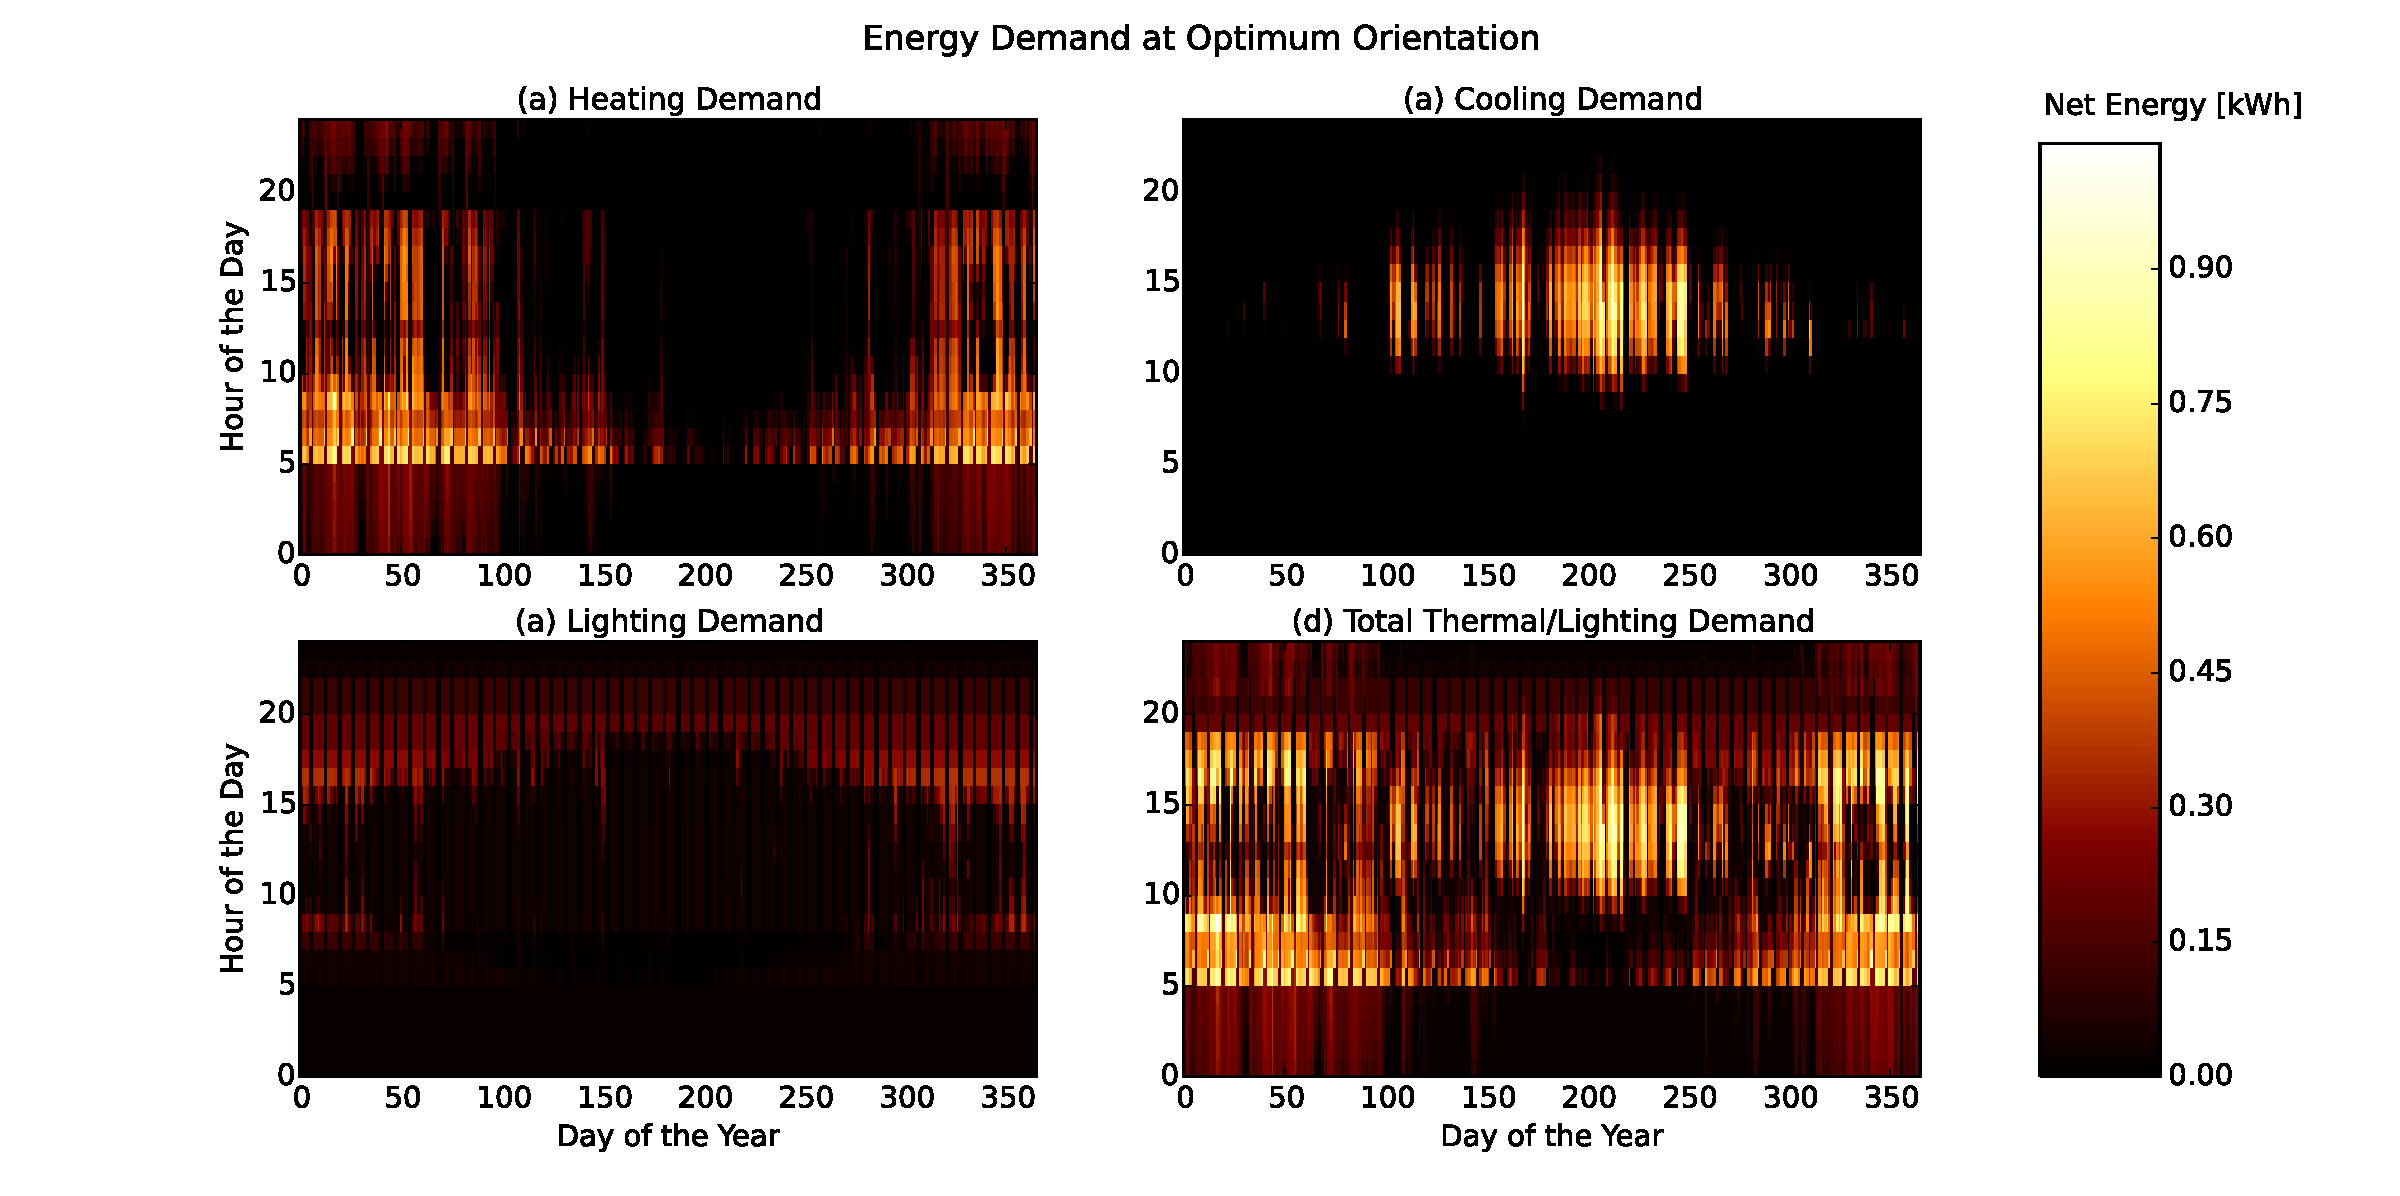
\includegraphics[width=\textwidth, trim= 0cm 0cm 0cm 0cm,clip]{DIVAe2}
		\caption{Carpet plots detailing the energy consumption during every hour of the year for the (a) heating demand, (b) cooling demand, (c) lighting demand, and (d) total building energy demand.}
		\label{f:DIVAe}
		\end{center}
	\end{figure*}
	


\section{Further Visualisations of Radiation and PV results}
\label{a:PV}

	The results of Sections \ref{s:baseCase} and \ref{s:compareSunTracking} were further visualised as can be seen in the following. Figure \ref{f:PV_angles} compares the angles that optimise PV electricity production with the angles that optimise the total radiation on the panels. The difference in the optimising angles can nicely be seen when comparing them side by side. While the radiation optimisation yields a symmetric pattern, the PV electricity production uses different angles, mainly in the afternoon. Figures \ref{f:PV_power} and \ref{f:PV_efficiency} correspond to the summarising Figure \ref{f:compareSuntracking}, but also show the actual difference in the power production and the efficiency, respectively. 

	\begin{figure*}[hb]
		\begin{center}
		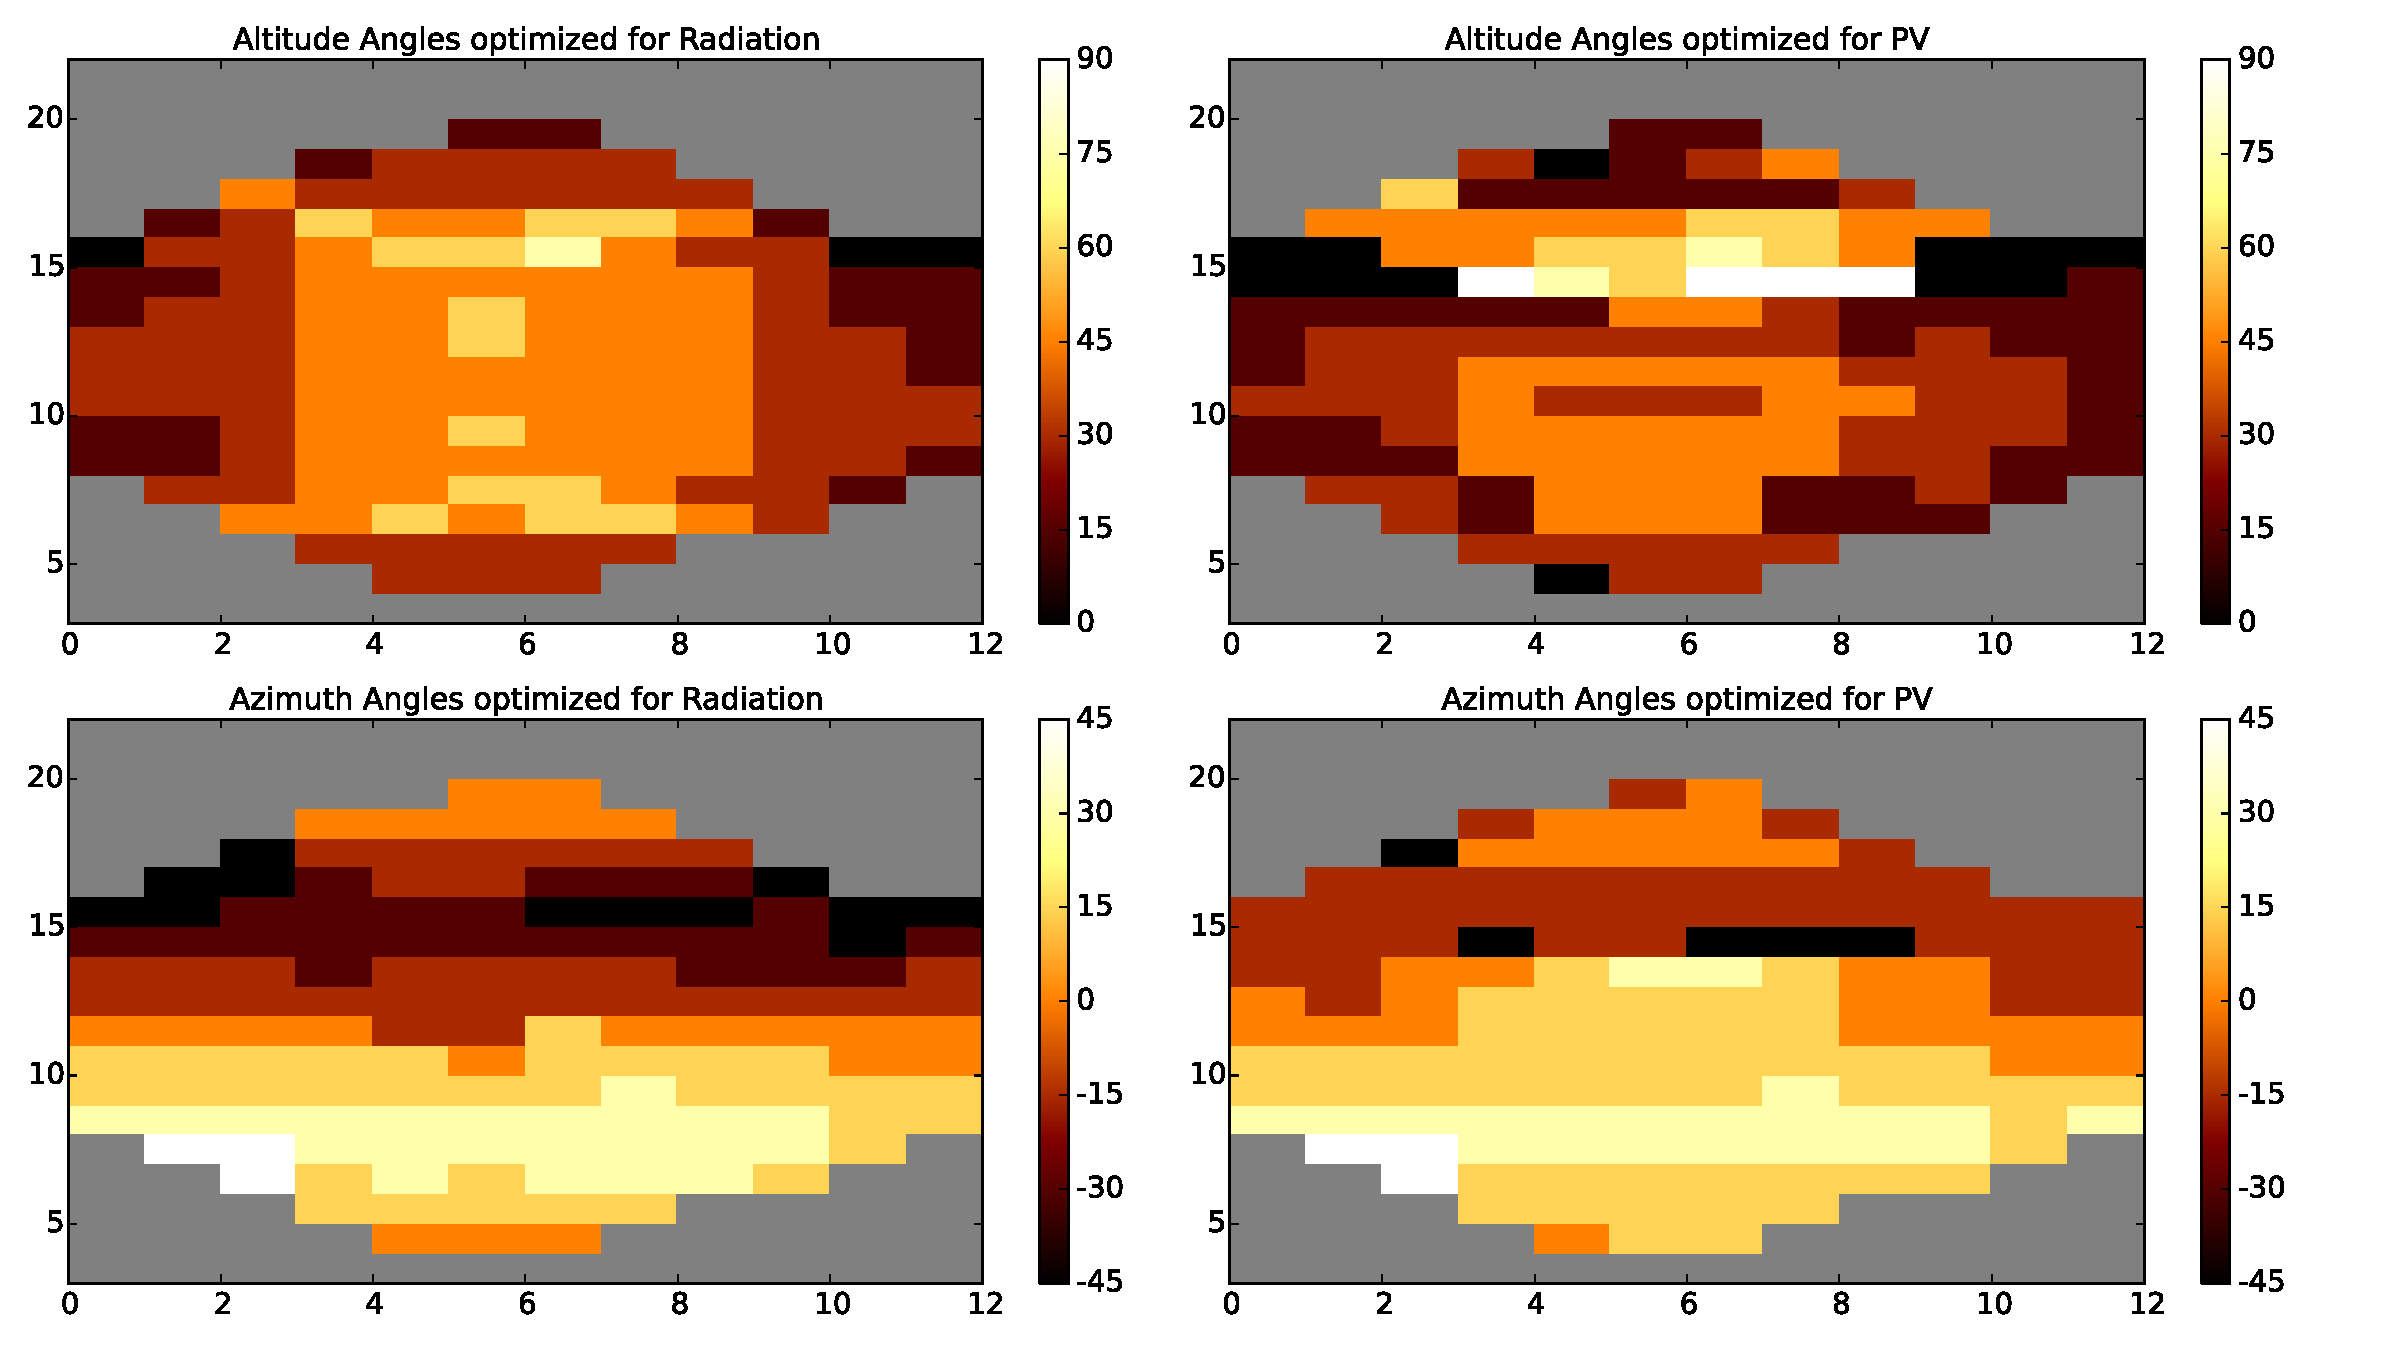
\includegraphics[width=\textwidth, trim= 0cm 0cm 0cm 0cm,clip]{PV_angles2}
		\caption{Angle visulisations, that optimise the altitude (top) and azimuth (bottom) angles for radiation (left) and PV electricity production (right). While the Radiation optimisation yields a symmetric pattern, the PV electricity optimisation deviates from the pattern that optimises the radiation in order to minimise longitudinal shading on the panels.}
		\label{f:PV_angles}
		\end{center}
	\end{figure*}

	\begin{figure*}
		\begin{center}
		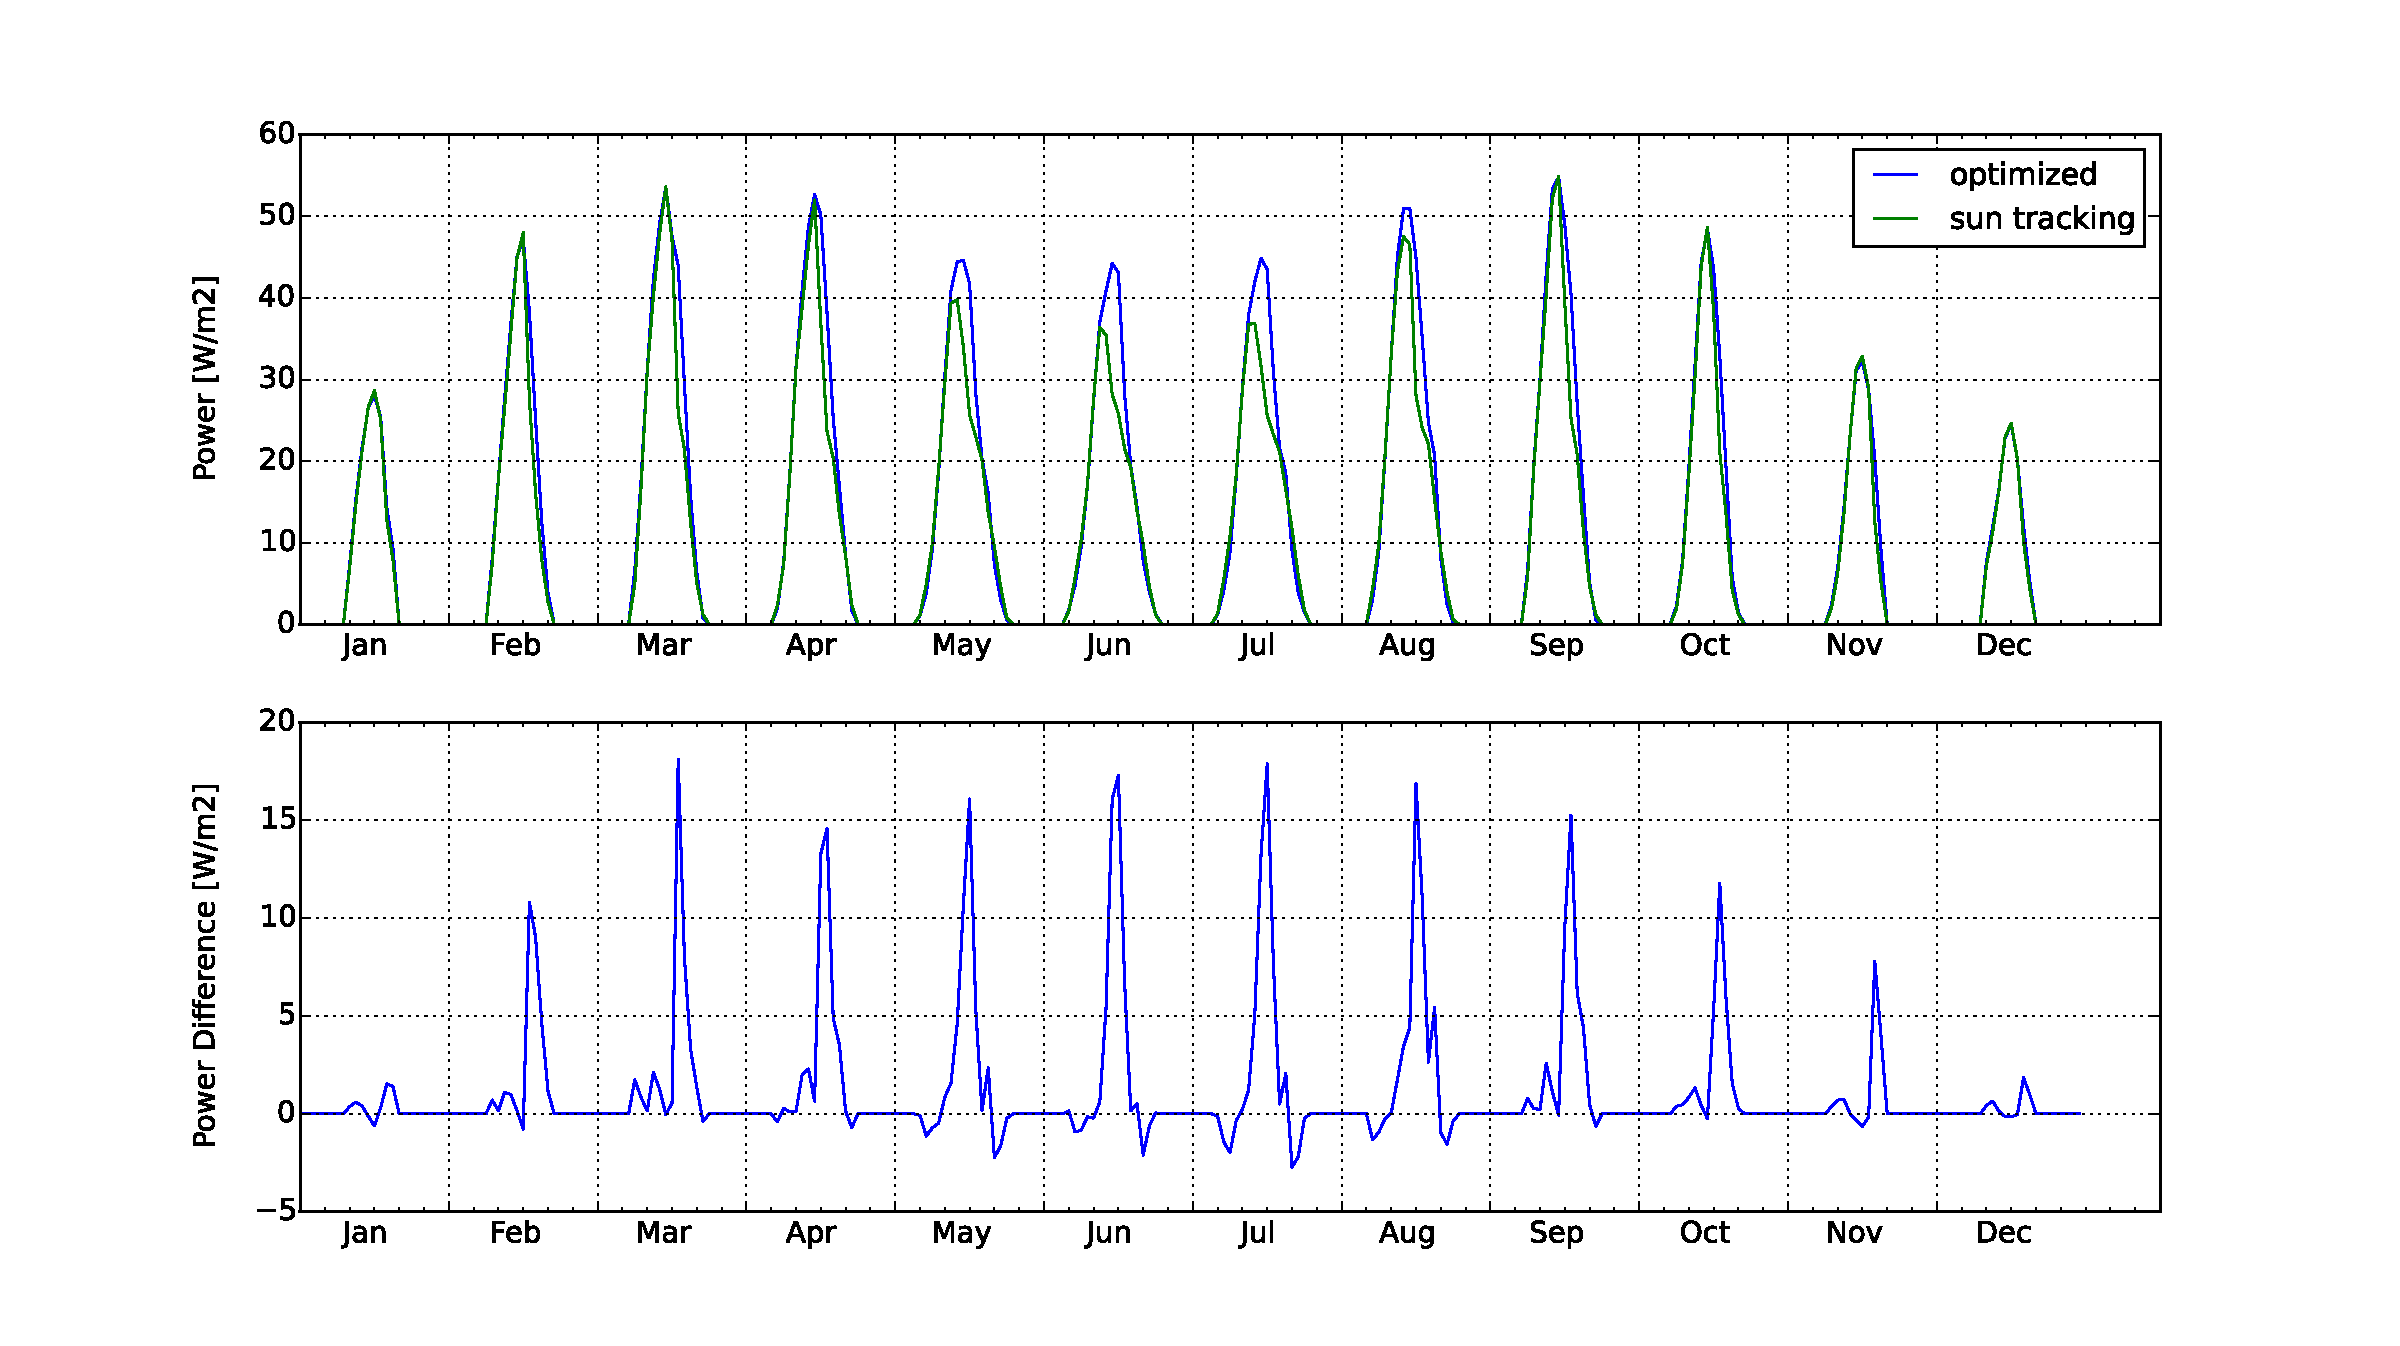
\includegraphics[width=\textwidth, trim= 3cm 0cm 2cm 2cm,clip]{PV_power}
		\caption{Comparison of PV electricity production with sun tracking to optimised solution. Top: Average power output for every month of the year. Bottom: Corresponding power difference. The difference is especially high during noon and in the afternoon.}
		\label{f:PV_power}
		\end{center}
	\end{figure*}

	\begin{figure*}
		\begin{center}
		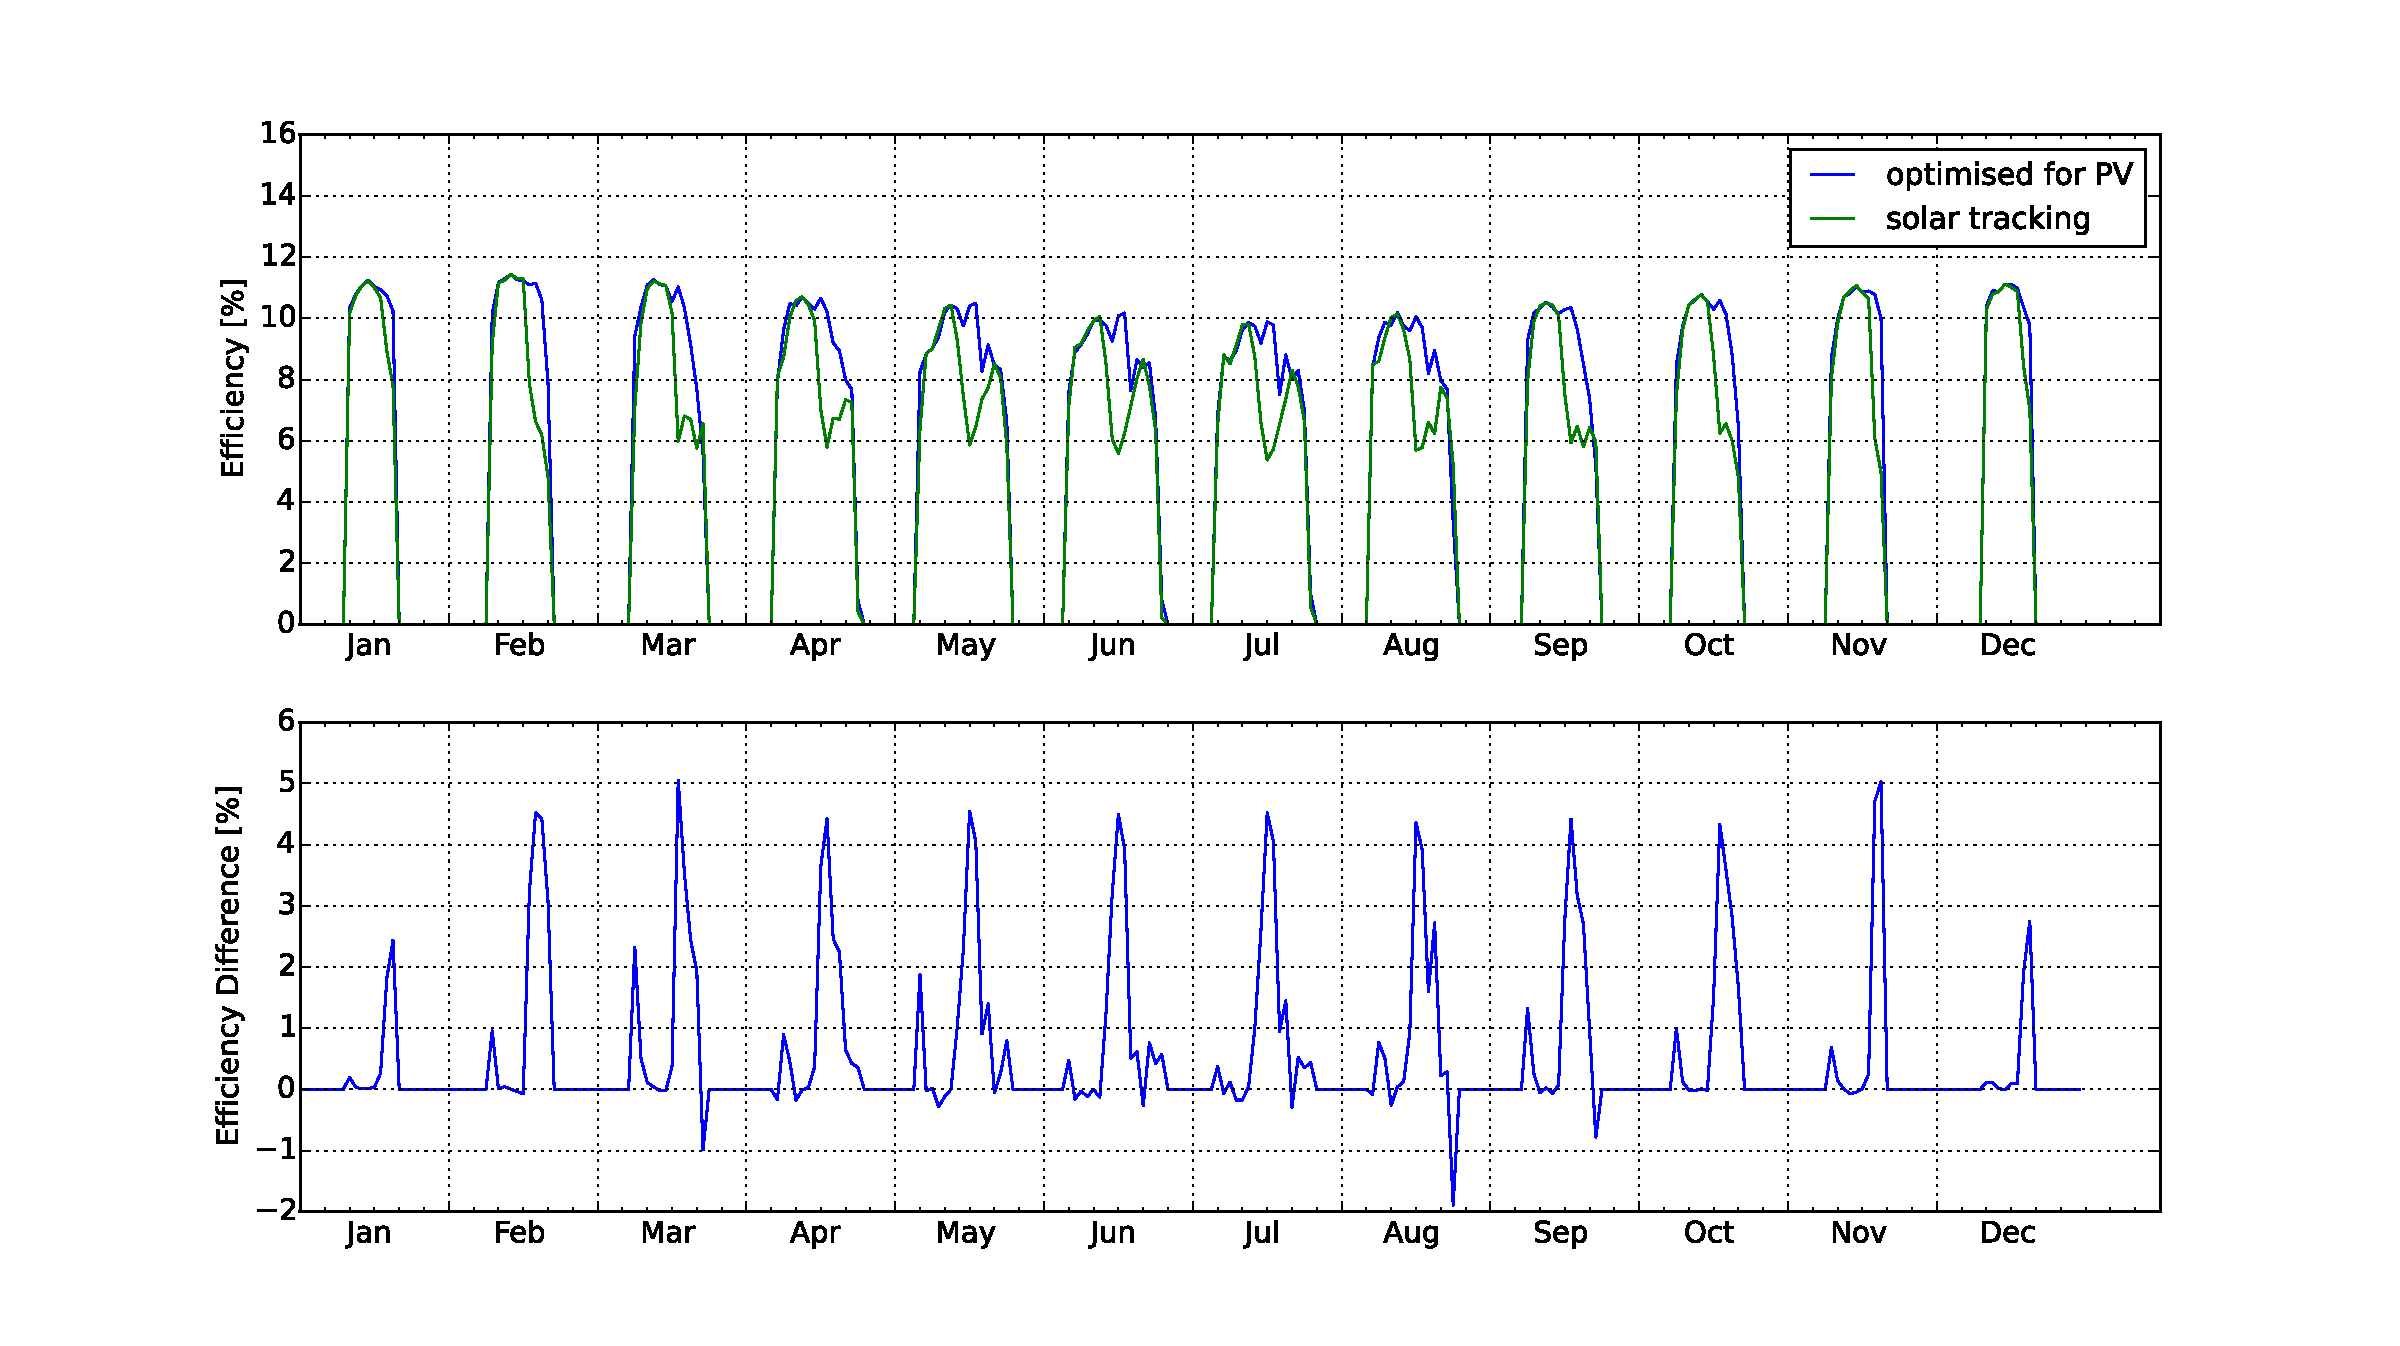
\includegraphics[width=\textwidth, trim= 3cm 0cm 2cm 2cm,clip]{PV_efficiency}
		\caption{Comparison of PV efficiency with sun tracking to optimised solution. Top: Average efficiency for every month of the year. Bottom: Corresponding efficiency difference. The difference is especially high during noon and in the afternoon.}
		\label{f:PV_efficiency}
		\end{center}
	\end{figure*}

	\cleardoublepage

\section{Tradeoffs Between Different Optimisation Strategies}
\label{a:tradeoffs}
	
	In order to visualize the tradeoffs between the different optimisation strategies, figures were created that show the influence of the different optimisation strategies on heating (figure \ref{f:tradeoff_H}), cooling (figure \ref{f:tradeoff_C}), lighting (figure \ref{f:tradeoff_L}), PV electricity (figure \ref{f:tradeoff_PV}), total building energy (figure \ref{f:tradeoff_HCL}) and net energy (figure \ref{f:tradeoff_E_tot}). Optimisation strategies were evaluated for heating (H), cooling (C), lighting (L), photovoltaic (PV), building energy demand (HCL), net energy demand (E\_tot), a combination of PV and cooling, and a fixed facade at a $45\degree$ altitude angle. The results from sections \ref{s:actuation} and \ref{s:tradeoffs} can be visualized here in more detail. It can clearly be seen, that while the cooling demand and the PV electricity production are strongly influenced by the actuation and the optimisation strategy, the lighting and heating have less fluctuations within the energy performance. 

	\begin{figure*}[hb]
		\begin{center}
		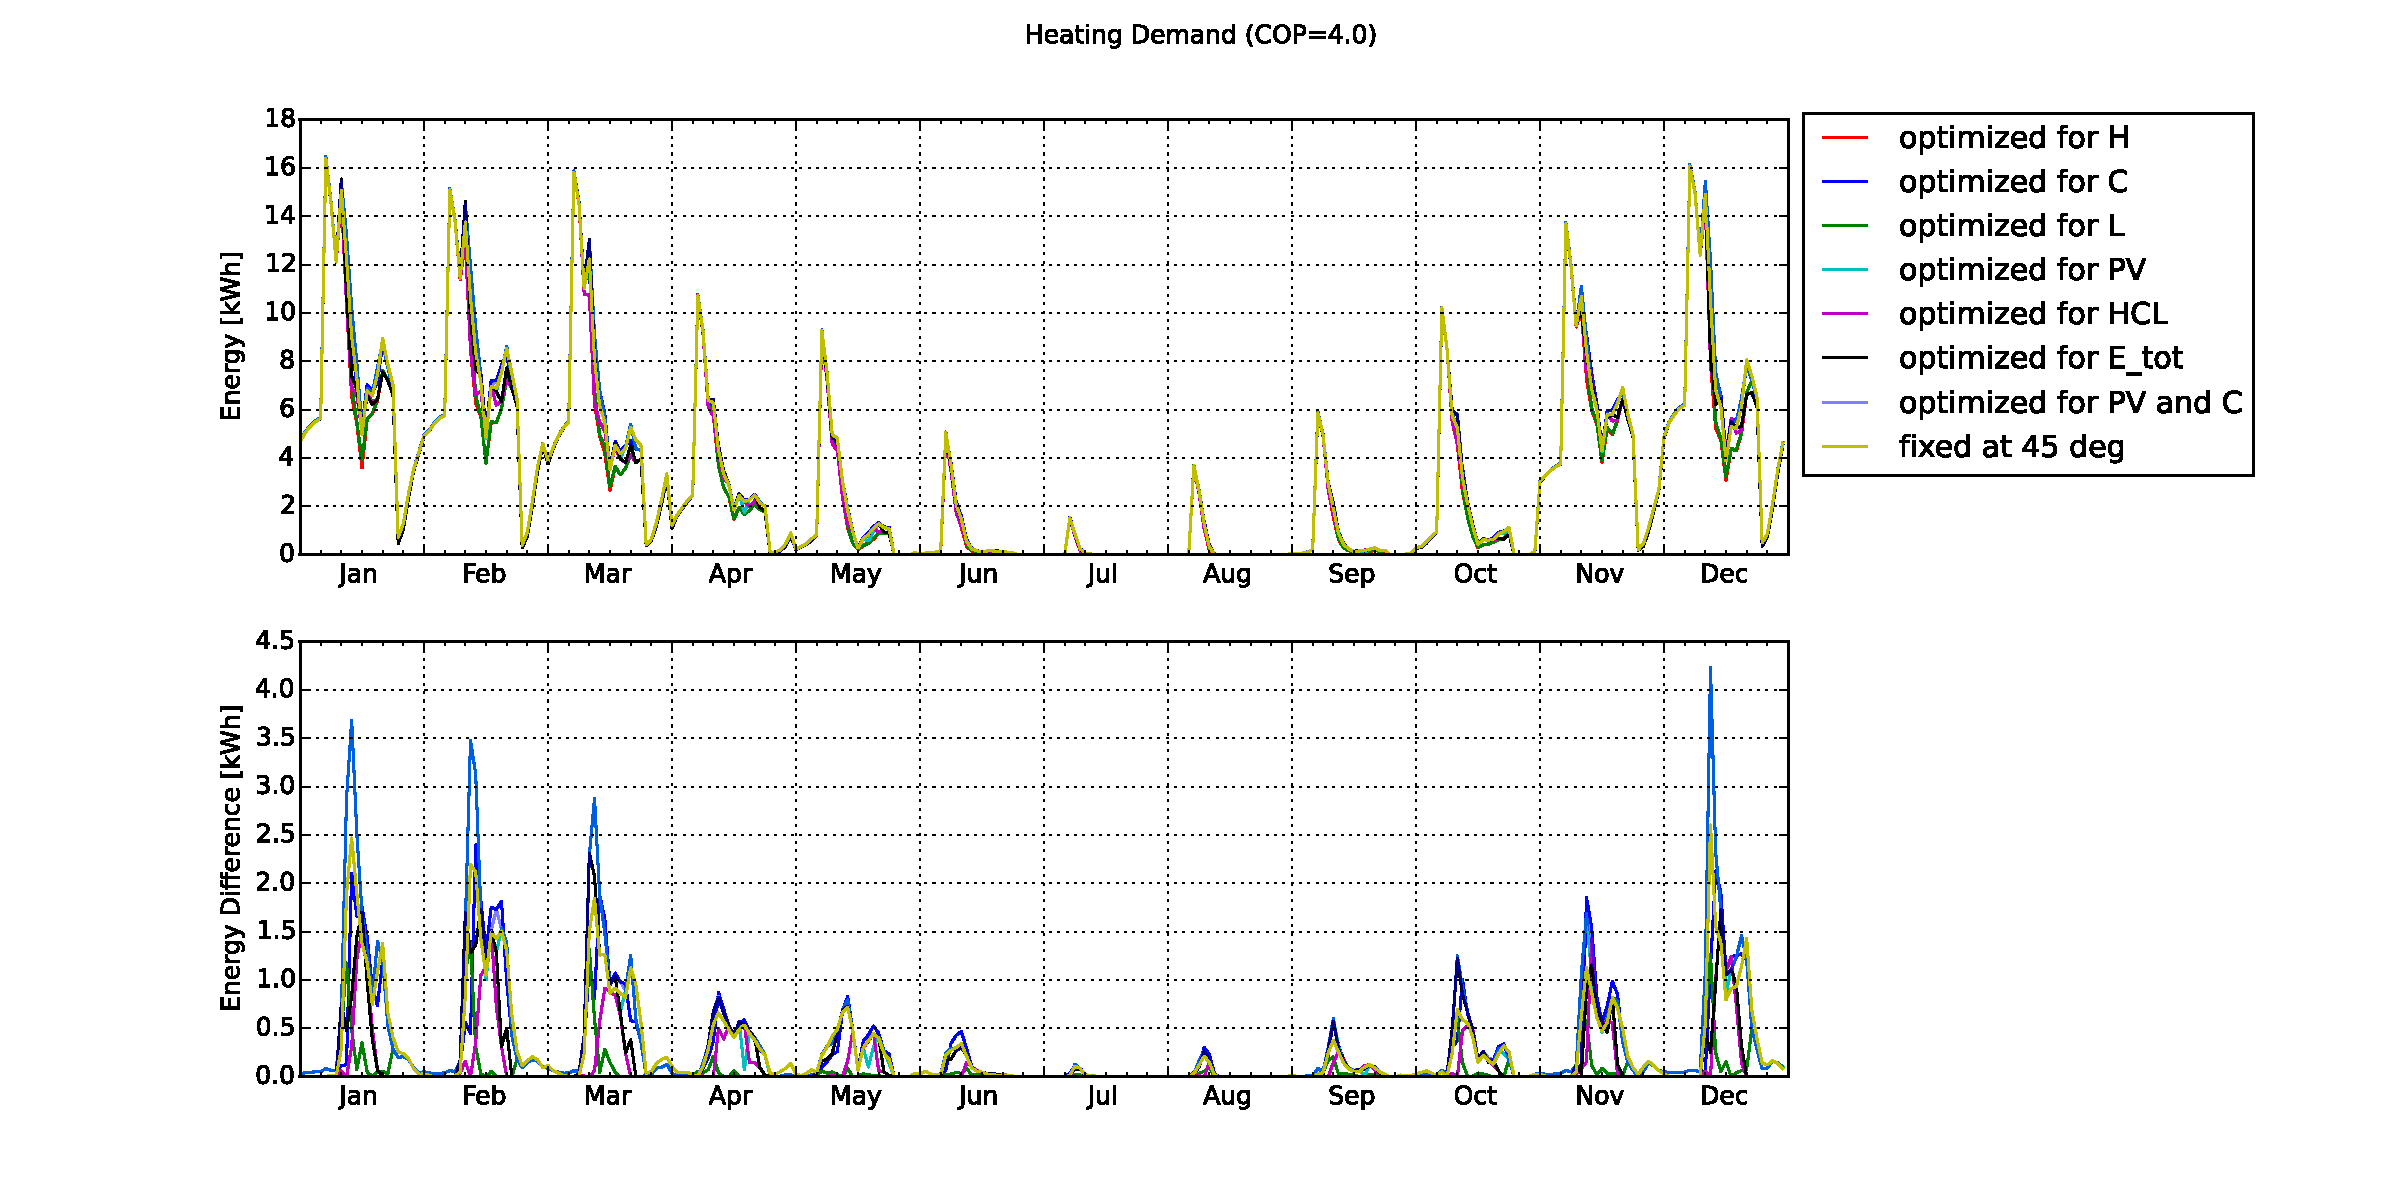
\includegraphics[width=\textwidth, trim= 3cm 0cm 2cm 0cm,clip]{tradeoff_H}
		\caption{Influence of optimisation strategy on heating demand. Top: Energy demand of heating in dependence of optimisation strategy. Bottom: Corresponding difference to heating optimisation.}
		\label{f:tradeoff_H}
		\end{center}
	\end{figure*}
	
	
	\begin{figure*}
		\begin{center}
		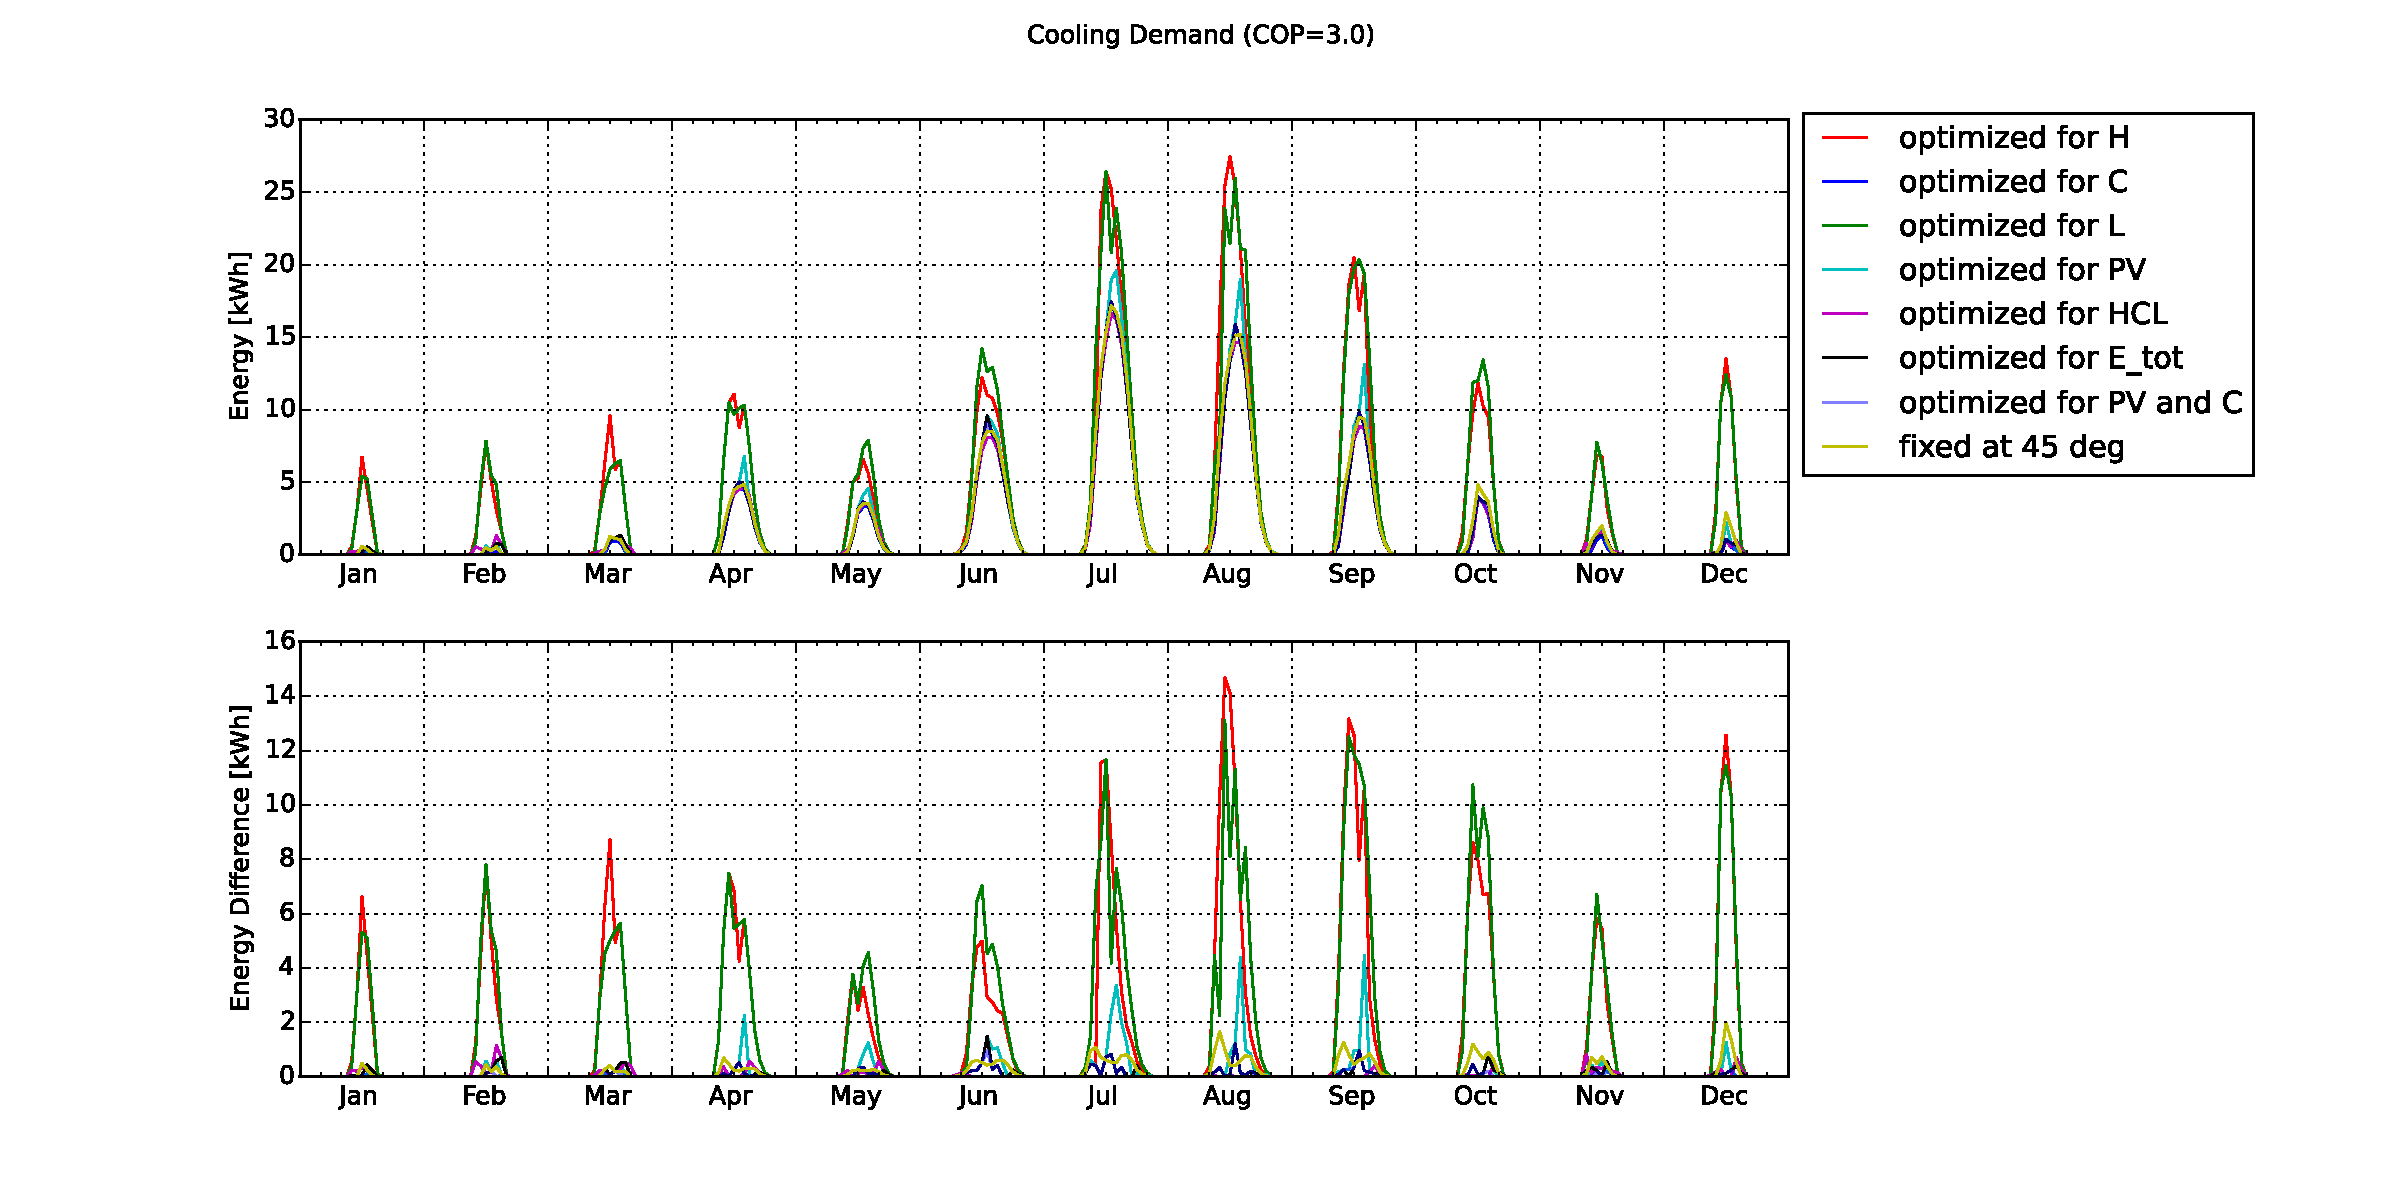
\includegraphics[width=\textwidth, trim= 3cm 0cm 2cm 0cm,clip]{tradeoff_C}
		\caption{Influence of optimisation strategy on cooling demand. Top: Energy demand of cooling in dependence of optimisation strategy. Bottom: Corresponding difference to cooling optimisation.}
		\label{f:tradeoff_C}
		\end{center}
	\end{figure*}

	\begin{figure*}
		\begin{center}
		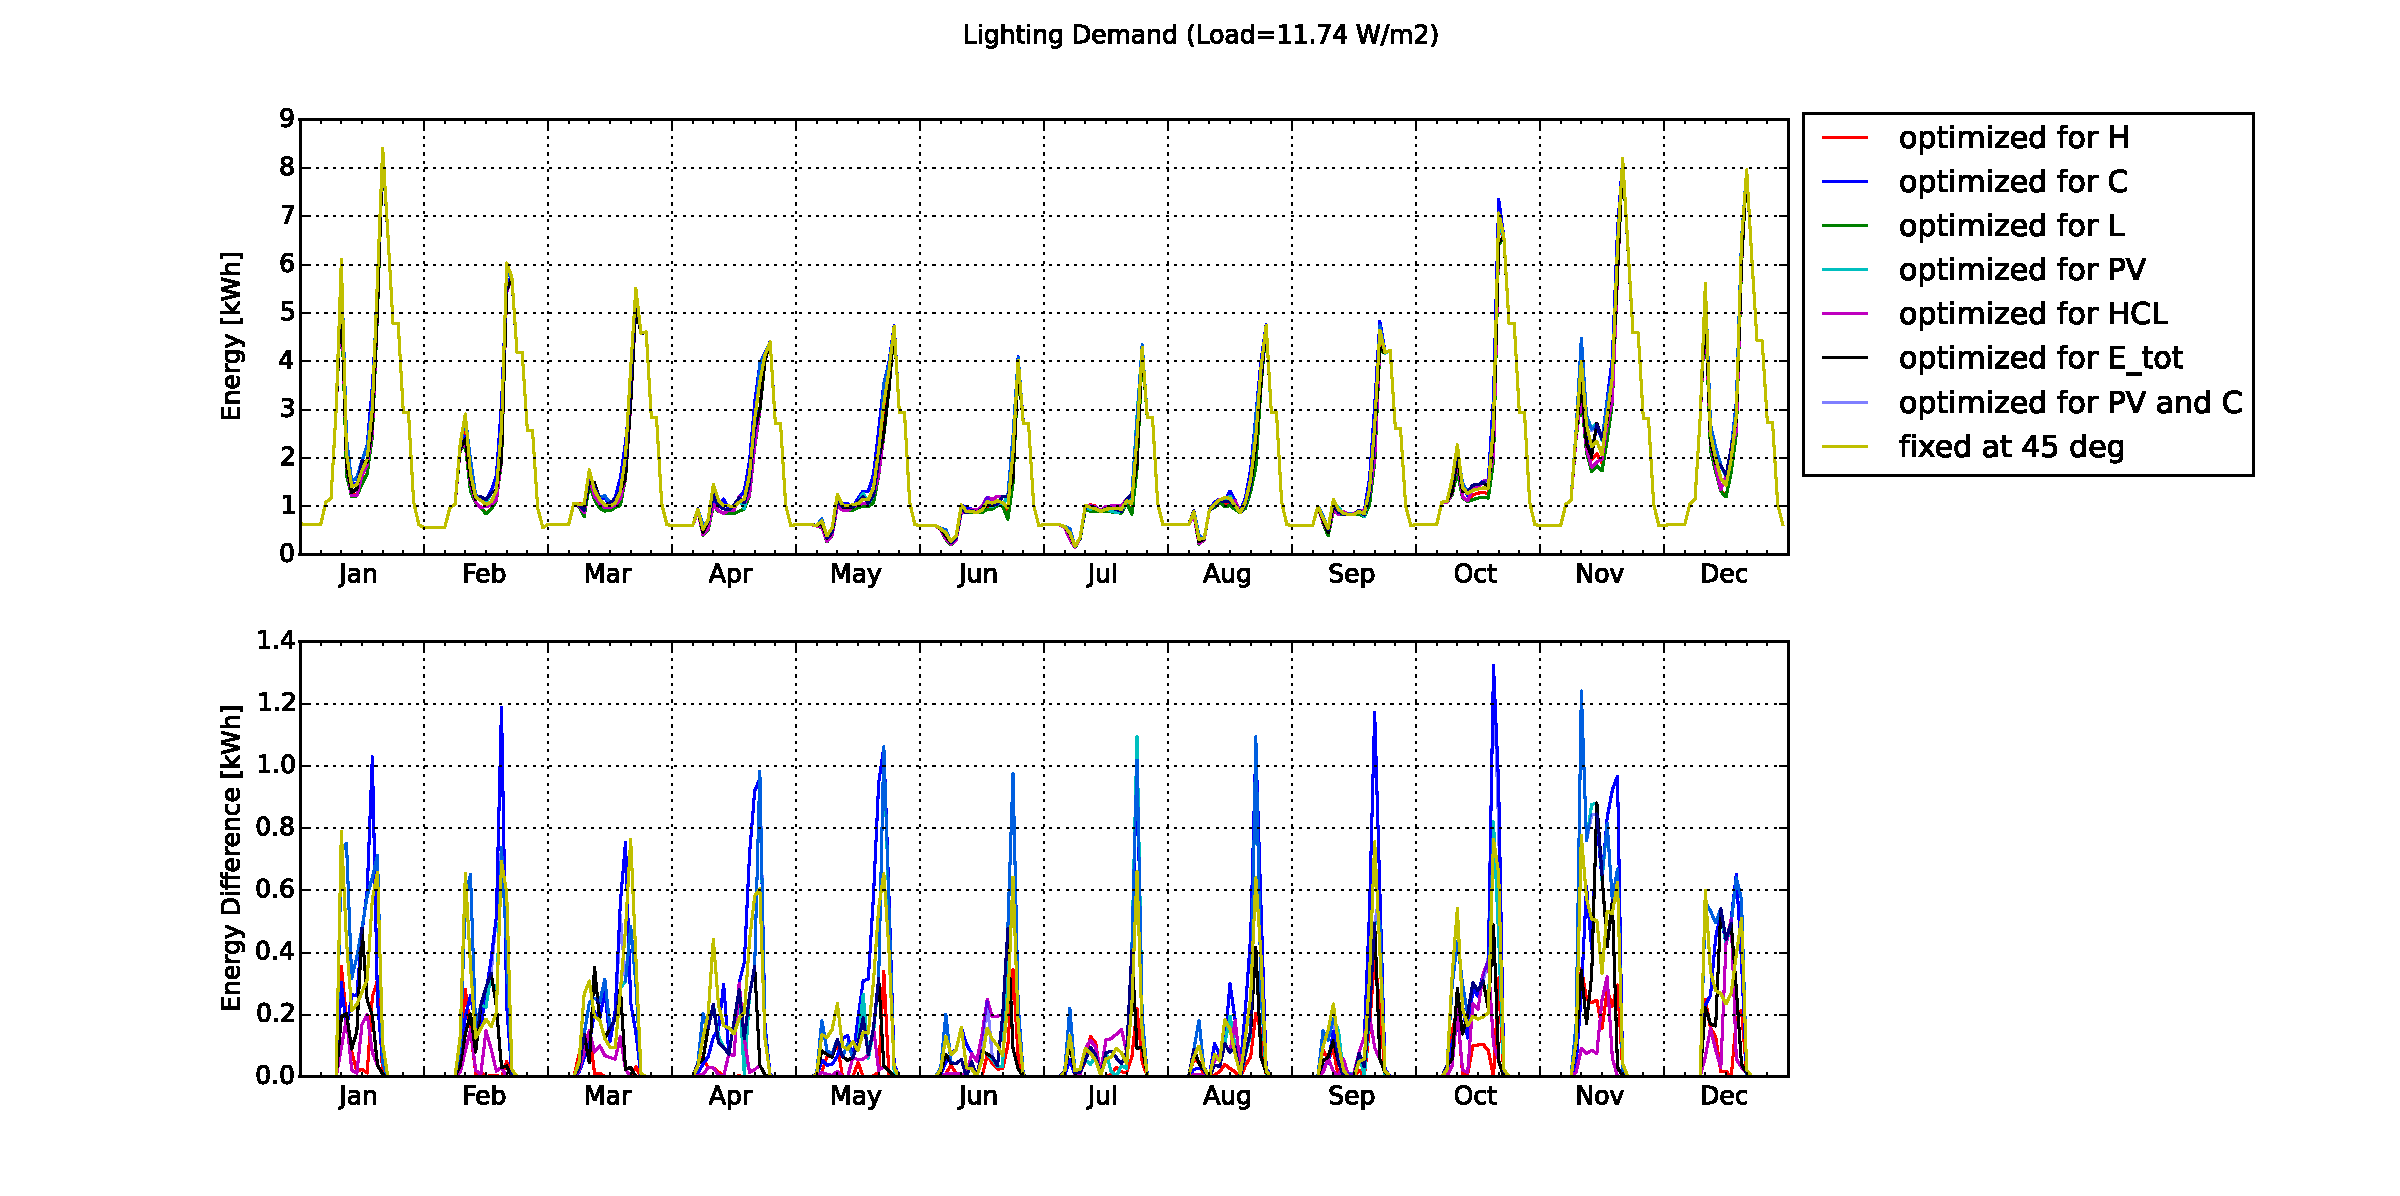
\includegraphics[width=\textwidth, trim= 3cm 0cm 2cm 0cm,clip]{tradeoff_L}
		\caption{Influence of optimisation strategy on lighting demand. Top: Energy demand of lighting in dependence of optimisation strategy. Bottom: Corresponding difference to lighting optimisation.}
		\label{f:tradeoff_L}
		\end{center}
	\end{figure*}

	\begin{figure*}
		\begin{center}
		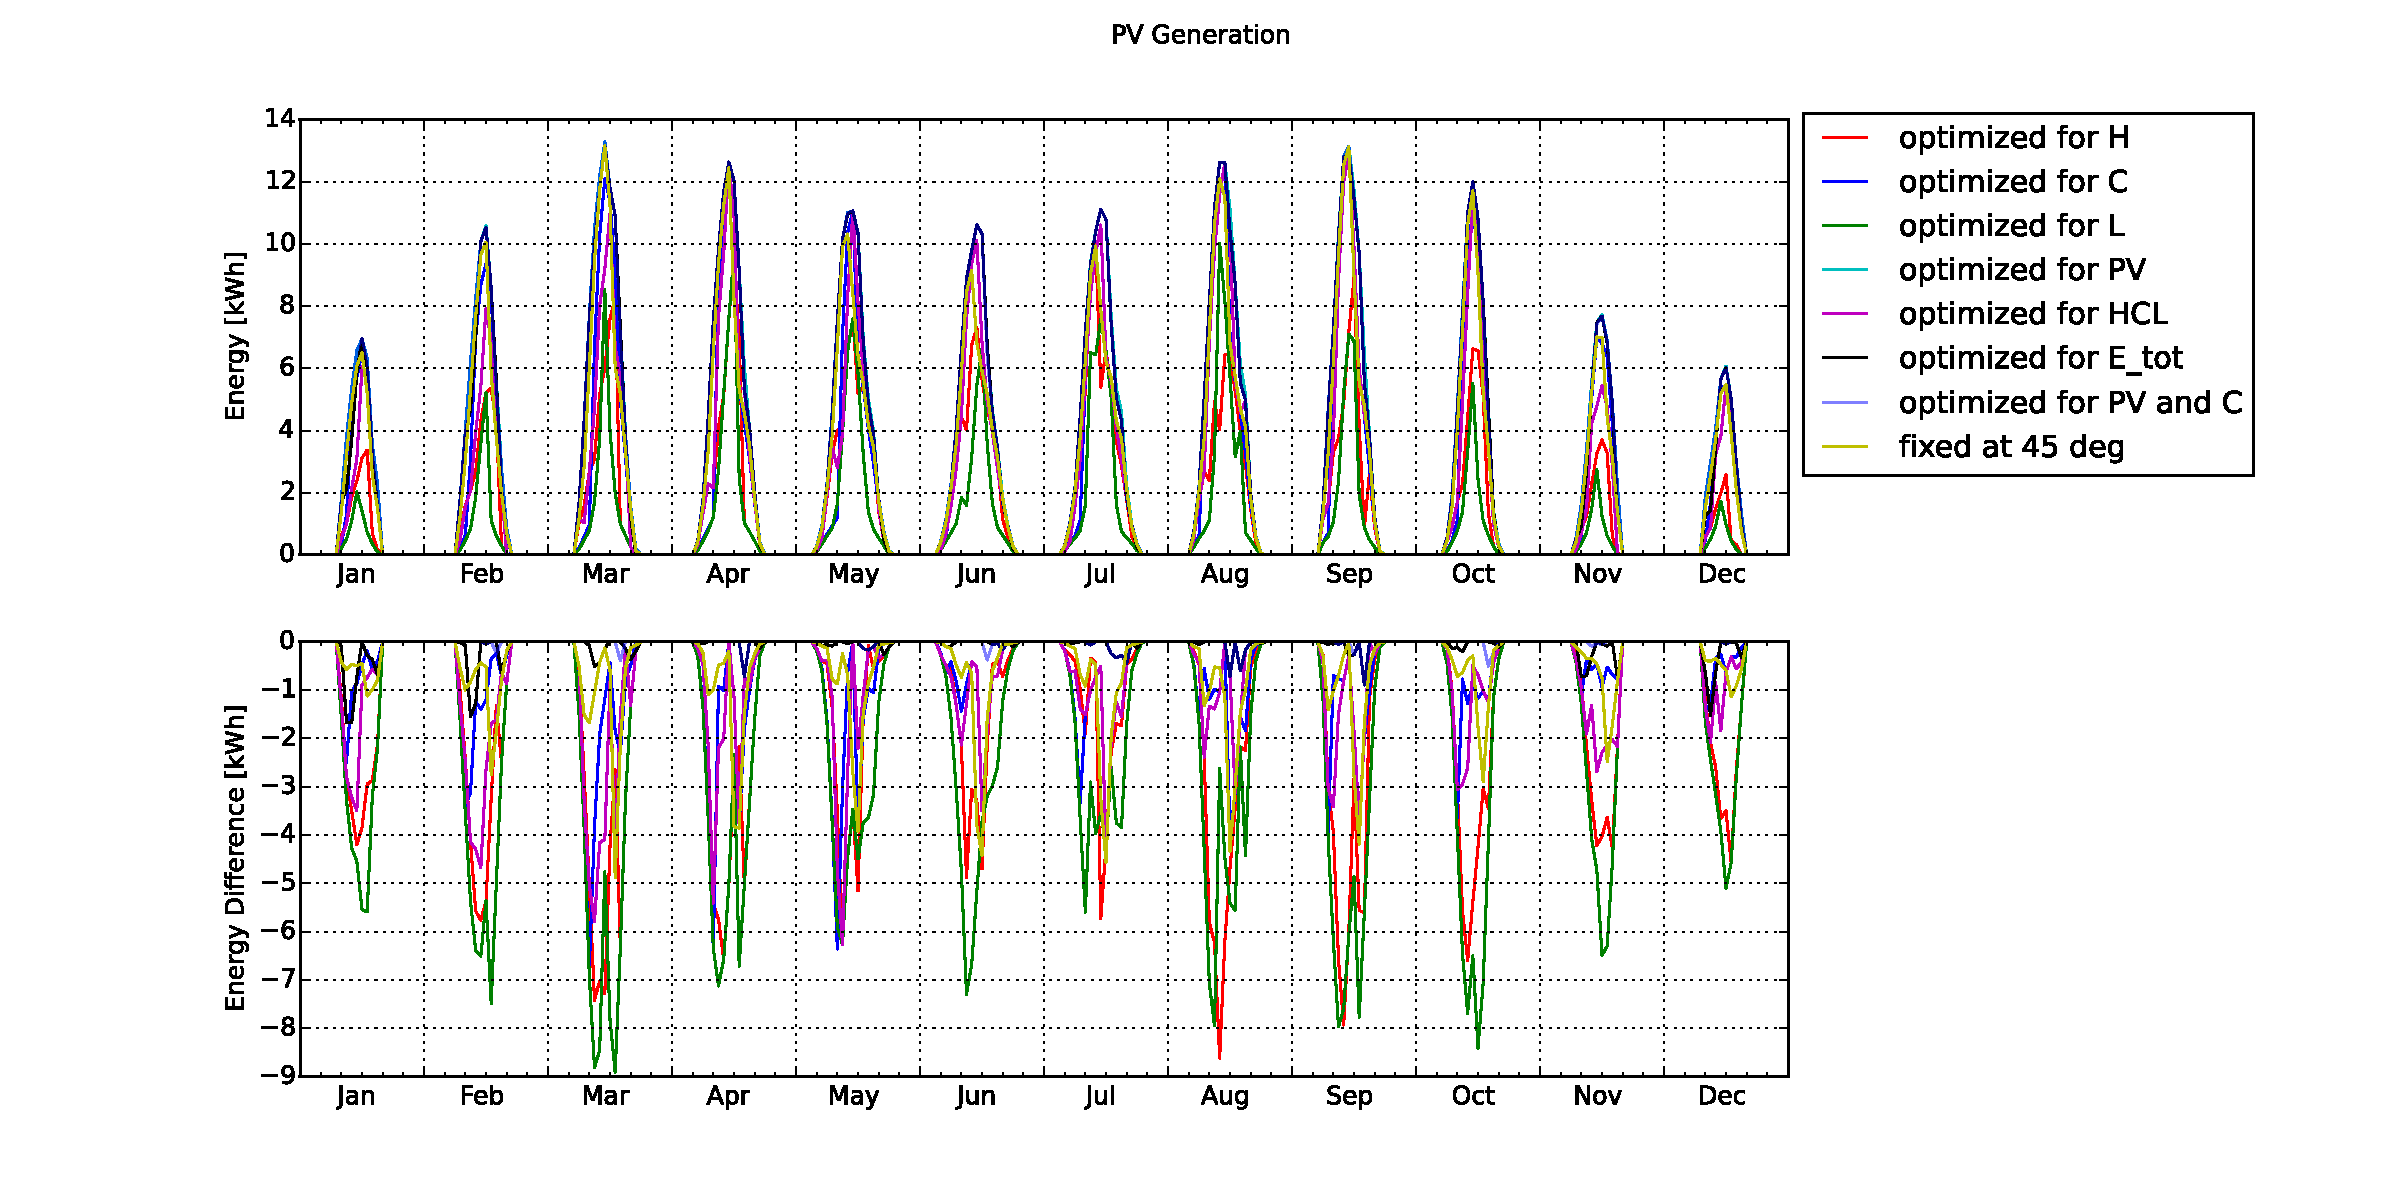
\includegraphics[width=\textwidth, trim= 3cm 0cm 2cm 0cm,clip]{tradeoff_PV}
		\caption{Influence of optimisation strategy on PV electricity production. Top: Energy demand of PV electricity production in dependence of optimisation strategy (negative because production corresponds to a negative demand). Bottom: Corresponding difference to PV electricity optimisation.}
		\label{f:tradeoff_PV}
		\end{center}
	\end{figure*}

	\begin{figure*}
		\begin{center}
		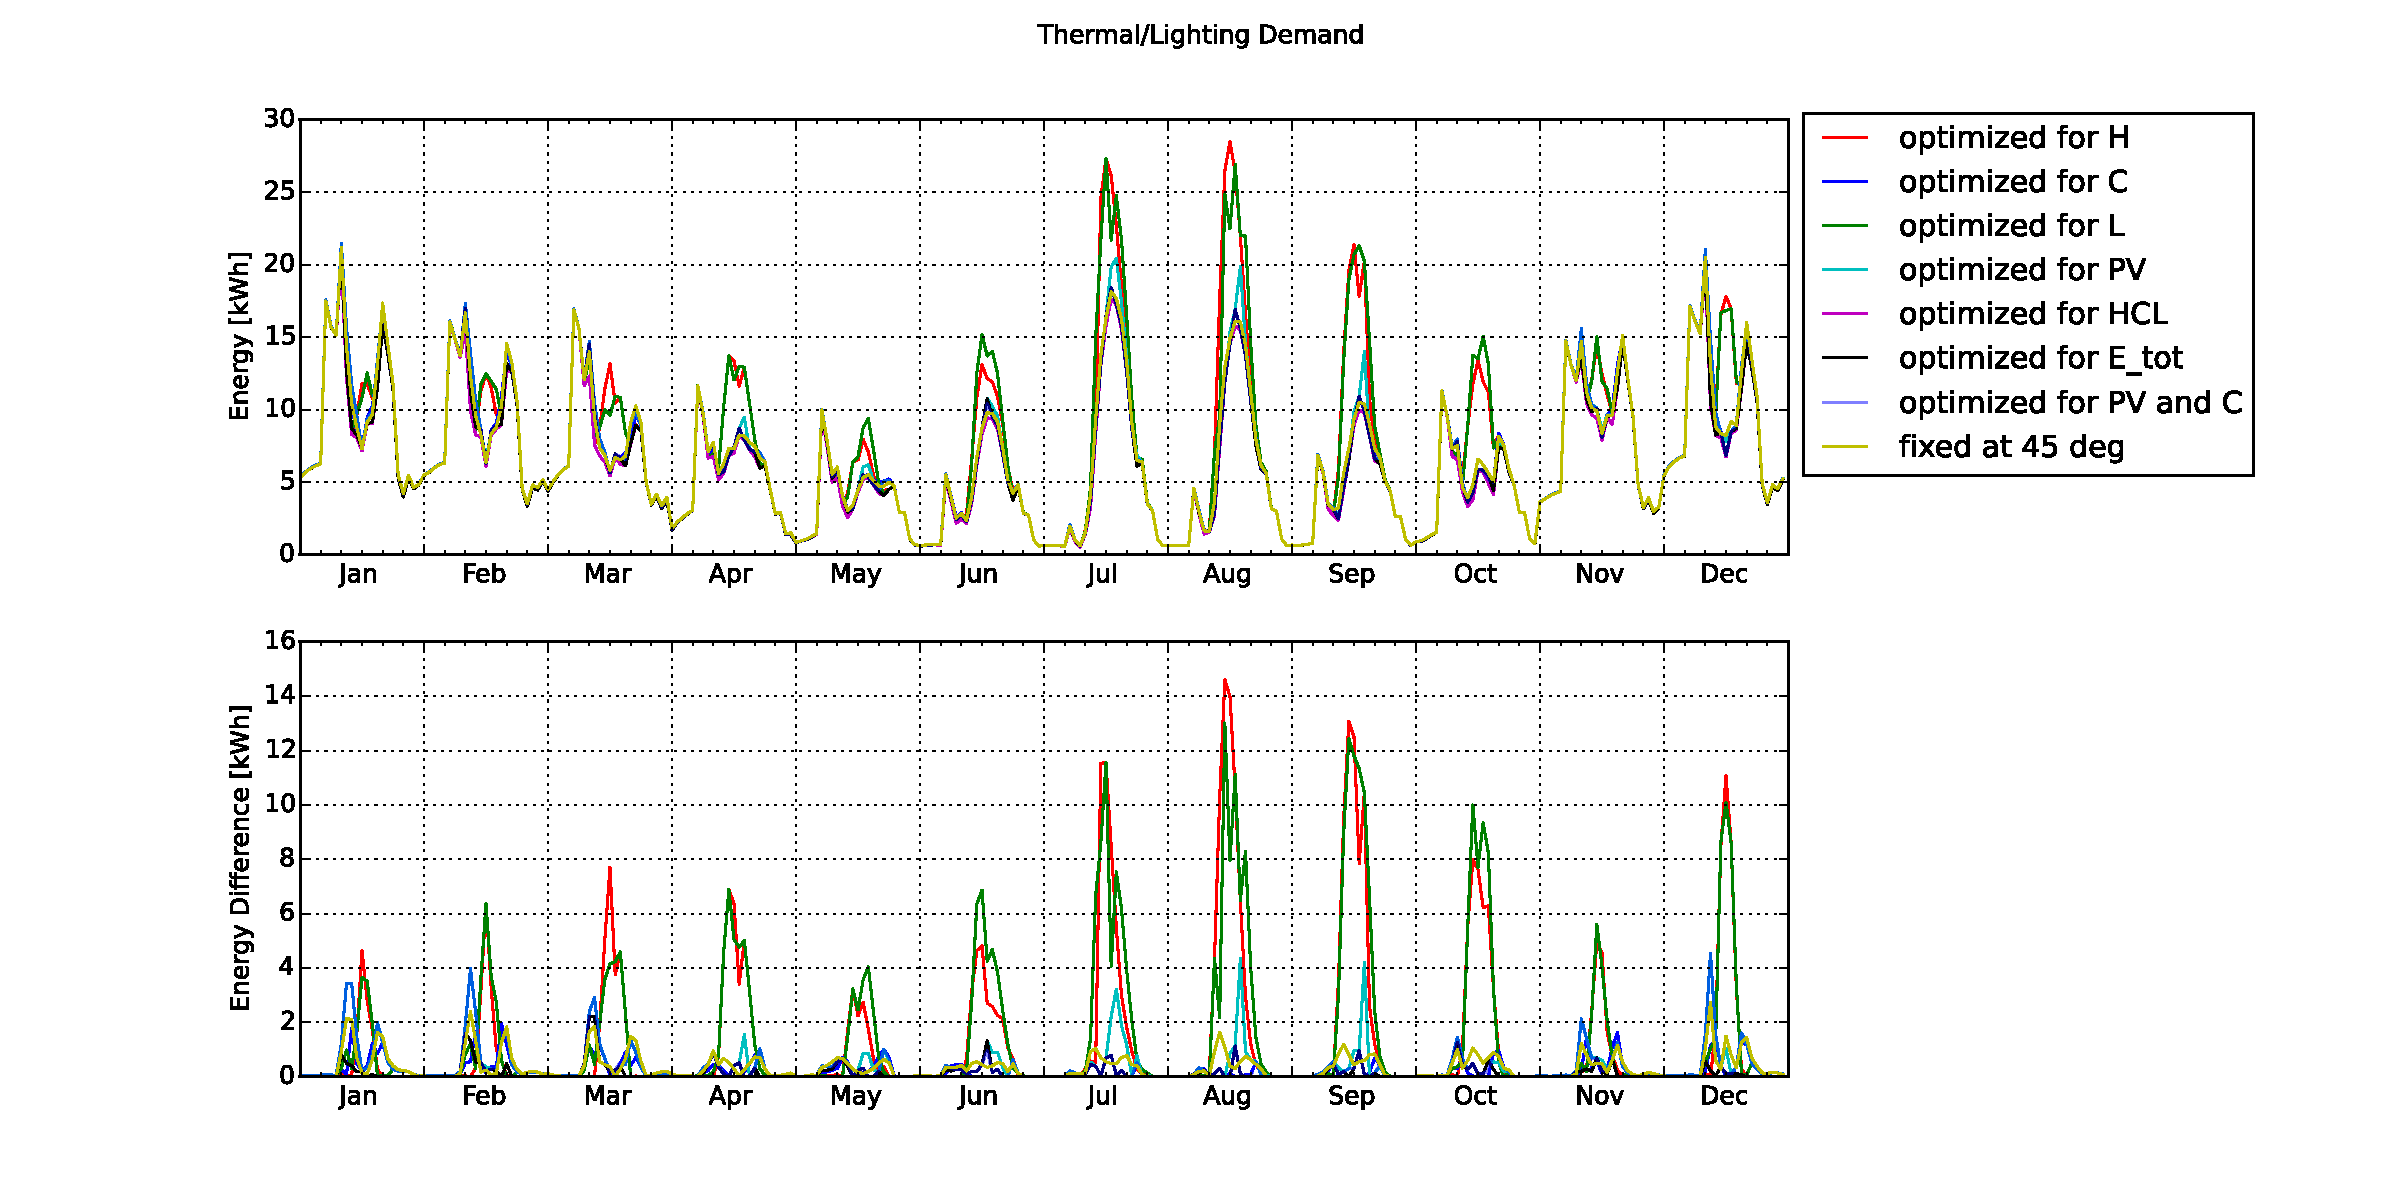
\includegraphics[width=\textwidth, trim= 3cm 0cm 2cm 0cm,clip]{tradeoff_HCL}
		\caption{Influence of optimisation strategy on building energy demand. Top: Building energy demand in dependence of optimisation strategy. Bottom: Corresponding difference to building energy demand optimisation.}
		\label{f:tradeoff_HCL}
		\end{center}
	\end{figure*}
	
	\begin{figure*}
		\begin{center}
		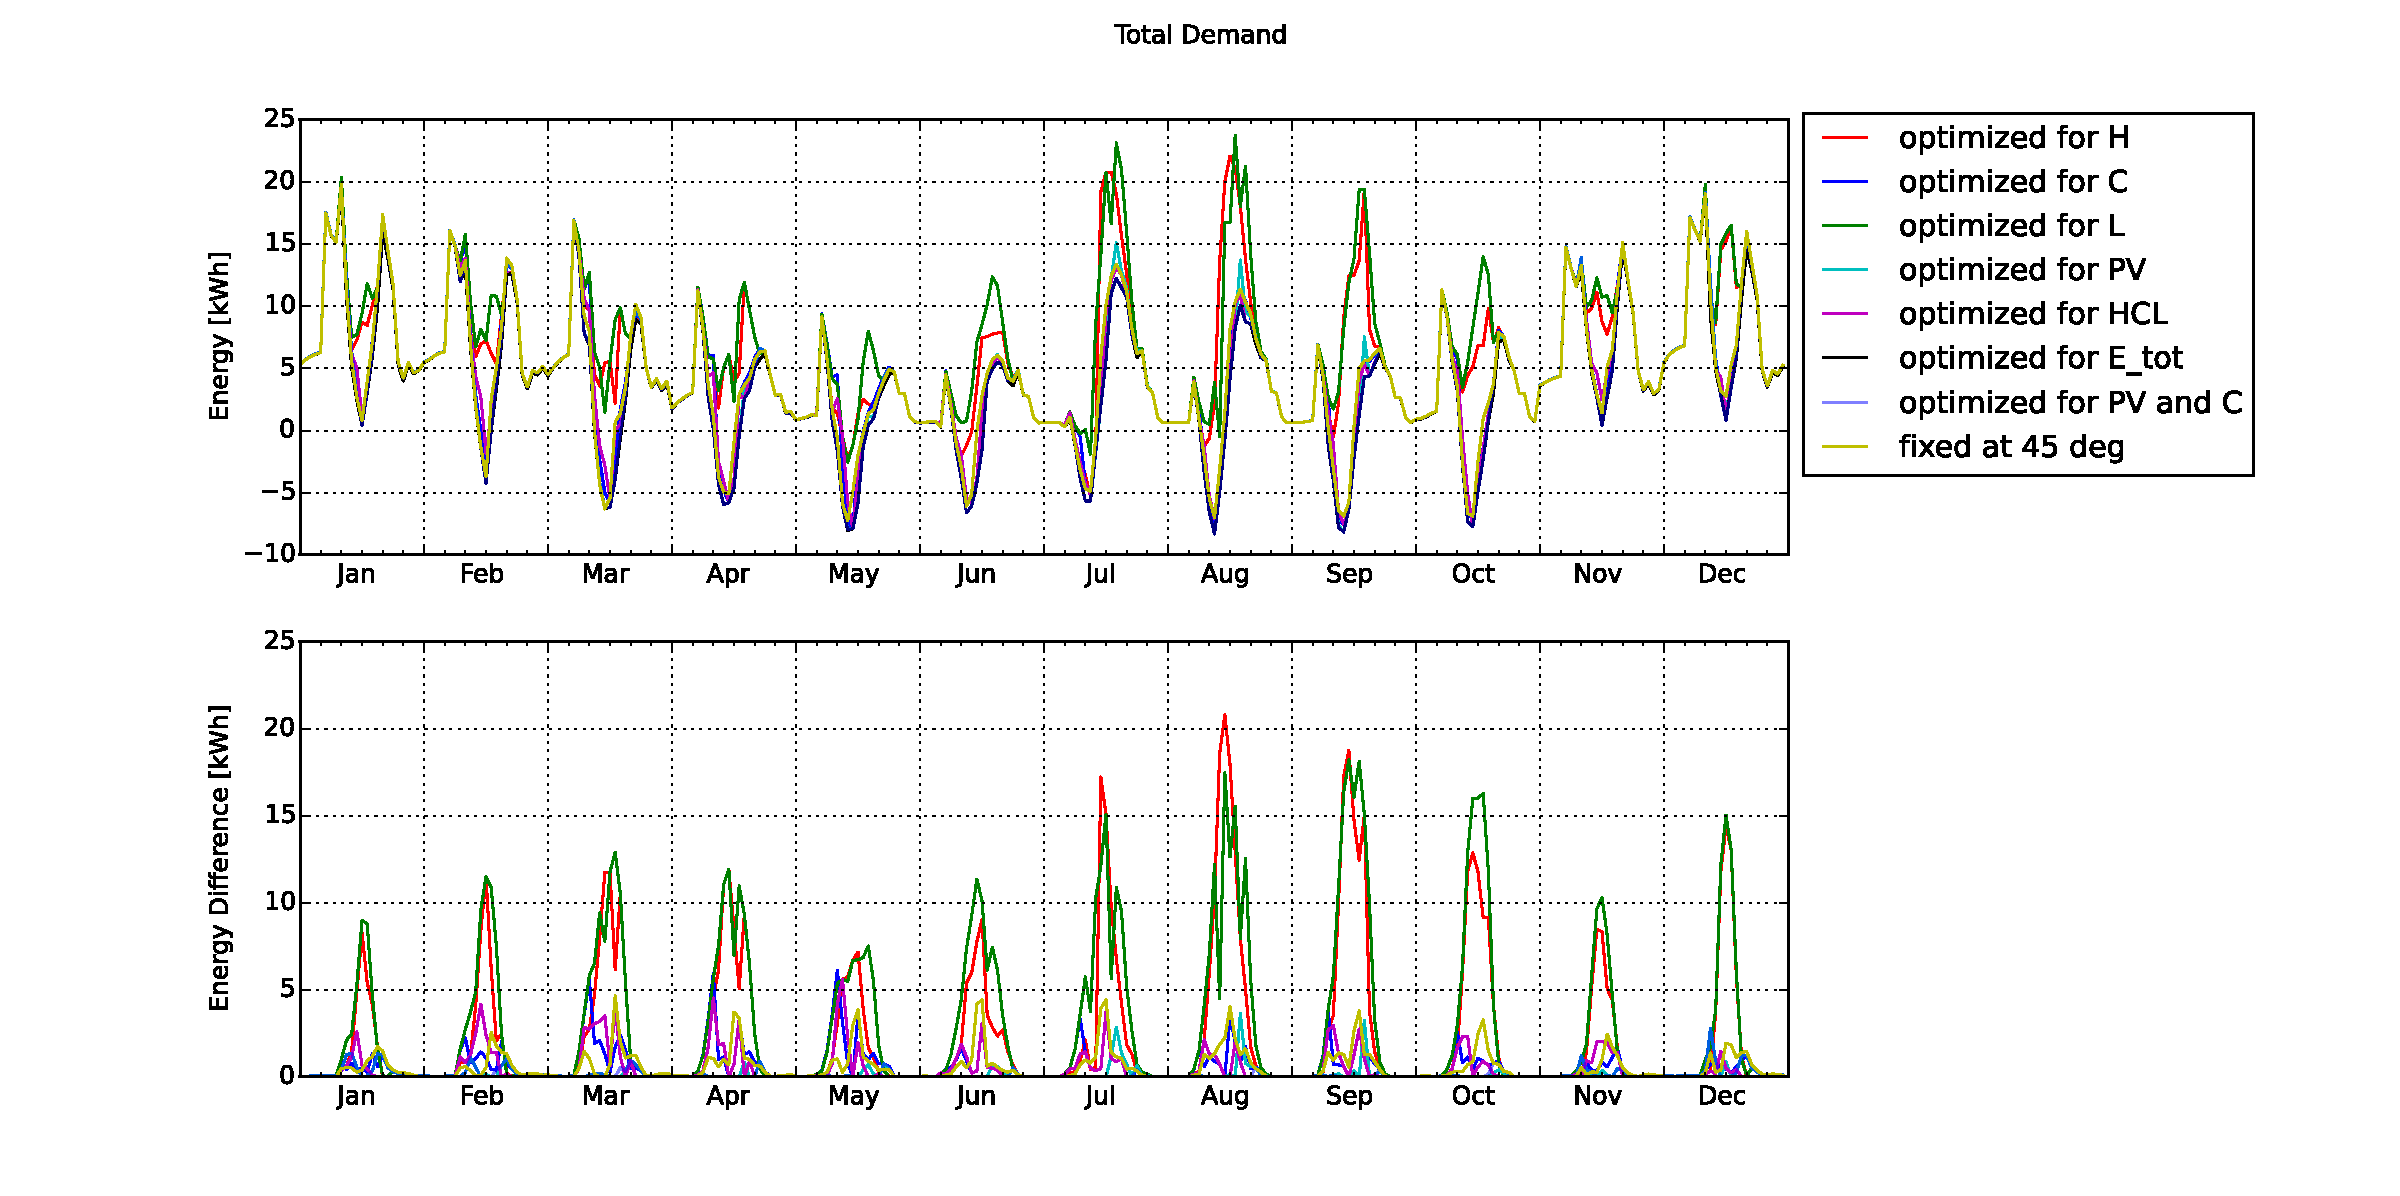
\includegraphics[width=\textwidth, trim= 3cm 0cm 2cm 0cm,clip]{tradeoff_E_tot}
		\caption{Influence of optimisation strategy on net energy demand including PV electricity production. Top: Net energy demand in dependence of optimisation strategy. Bottom: Corresponding difference to overall optimisation.}
		\label{f:tradeoff_E_tot}
		\end{center}
	\end{figure*}
	
	
	\begin{figure*}
		\begin{center}
		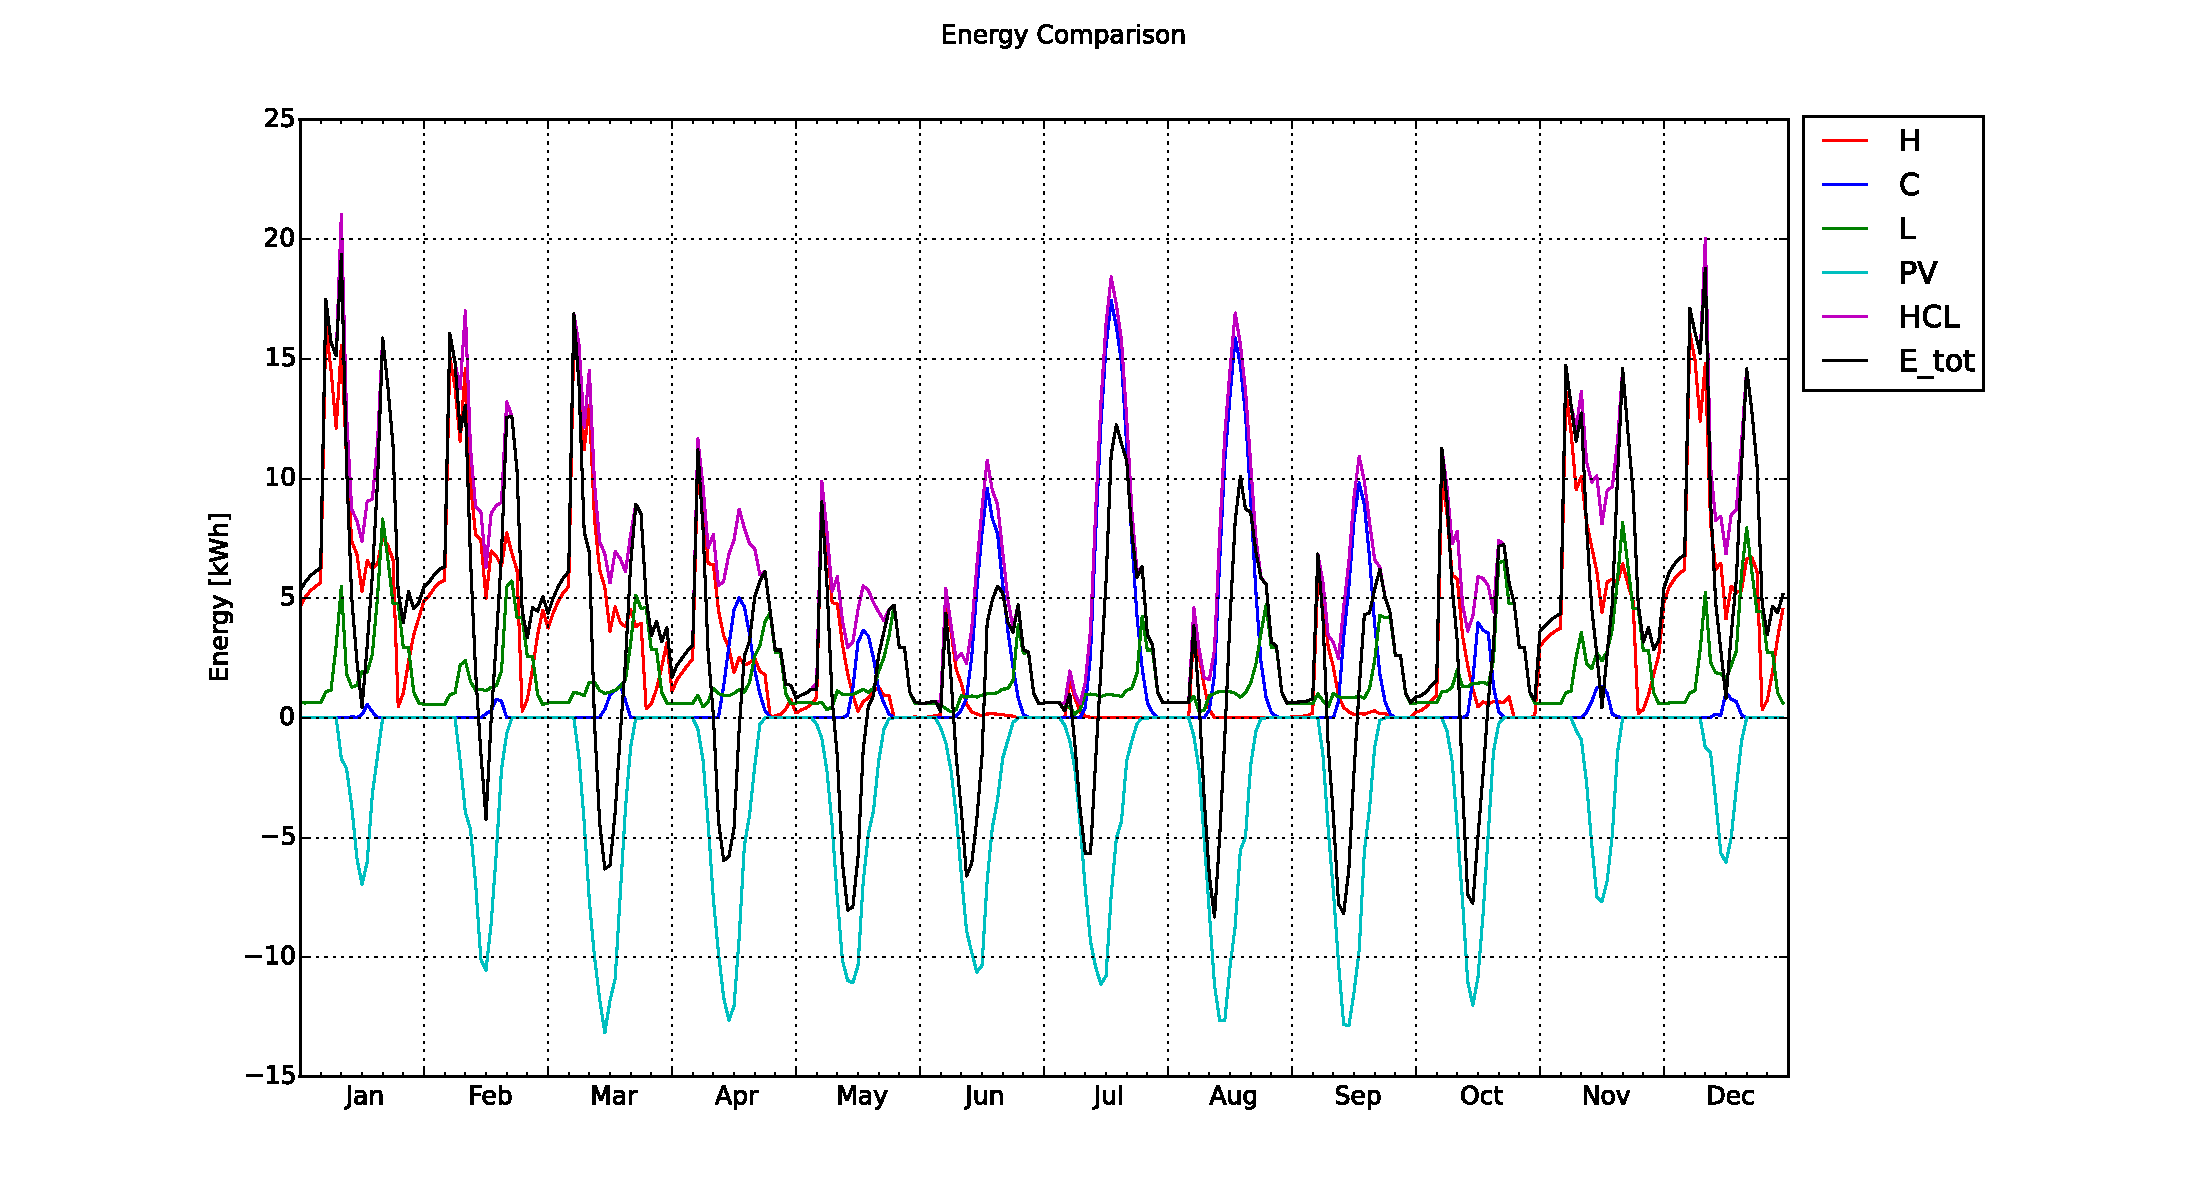
\includegraphics[width=\textwidth, trim= 3cm 0cm 2cm 0cm,clip]{energies}
		\caption{Energy demand distribution at overall optimization.}
		\label{f:energies}
		\end{center}
	\end{figure*}
